% This file was created (at least in part) by the script ParseMdtoLatex by Louis du Plessis
% (Available from https://github.com/taming-the-beast)

\documentclass[11pt]{article}
%%%%%%%%%%%%%%%%%%%%%%%%%%%%%%%%%%%%%%%%%%%%%%%%%%%%%%%%%%%%%%%
% DO NOT EDIT THIS FILE UNLESS YOU KNOW WHAT YOU ARE DOING!!! %
%%%%%%%%%%%%%%%%%%%%%%%%%%%%%%%%%%%%%%%%%%%%%%%%%%%%%%%%%%%%%%%

\usepackage[]{authblk}
\usepackage{graphicx}
\usepackage{color}
\usepackage{longtable}
\usepackage{hanging}
\usepackage{indentfirst}
\usepackage{setspace}
\usepackage{enumitem}
\usepackage{verbatim}
\usepackage{upgreek}
\usepackage{framed}
\usepackage{textcomp}
\usepackage{url}
\usepackage{soul}
\usepackage{amsmath, amsfonts,amssymb,mathrsfs}
\usepackage{fancyhdr}
\usepackage[compact]{titlesec}
\usepackage[T1]{fontenc}
\usepackage{lmodern}

\usepackage[backend=bibtex,hyperref=true,citestyle=authoryear,bibstyle=authortitle,firstinits=true,terseinits=true,doi=false,url=false,eprint=false,maxbibnames=10,maxcitenames=2]{biblatex}
\DeclareCiteCommand{\cite}
  {\usebibmacro{prenote}}
  {\usebibmacro{citeindex}%
   \printtext[bibhyperref]{\usebibmacro{cite}}}
  {\multicitedelim}
  {\usebibmacro{postnote}}

\DeclareCiteCommand*{\cite}
  {\usebibmacro{prenote}}
  {\usebibmacro{citeindex}%
   \printtext[bibhyperref]{\usebibmacro{citeyear}}}
  {\multicitedelim}
  {\usebibmacro{postnote}}

\DeclareCiteCommand{\parencite}[\mkbibparens]
  {\usebibmacro{prenote}}
  {\usebibmacro{citeindex}%
    \printtext[bibhyperref]{\usebibmacro{cite}}}
  {\multicitedelim}
  {\usebibmacro{postnote}}

\DeclareCiteCommand*{\parencite}[\mkbibparens]
  {\usebibmacro{prenote}}
  {\usebibmacro{citeindex}%
    \printtext[bibhyperref]{\usebibmacro{citeyear}}}
  {\multicitedelim}
  {\usebibmacro{postnote}}

\DeclareCiteCommand{\footcite}[\mkbibfootnote]
  {\usebibmacro{prenote}}
  {\usebibmacro{citeindex}%
  \printtext[bibhyperref]{ \usebibmacro{cite}}}
  {\multicitedelim}
  {\usebibmacro{postnote}}

\DeclareCiteCommand{\footcitetext}[\mkbibfootnotetext]
  {\usebibmacro{prenote}}
  {\usebibmacro{citeindex}%
   \printtext[bibhyperref]{\usebibmacro{cite}}}
  {\multicitedelim}
  {\usebibmacro{postnote}}

\DeclareCiteCommand{\textcite}
  {\boolfalse{cbx:parens}}
  {\usebibmacro{citeindex}%
   \printtext[bibhyperref]{\usebibmacro{textcite}}}
  {\ifbool{cbx:parens}
     {\bibcloseparen\global\boolfalse{cbx:parens}}
     {}%
   \multicitedelim}
  {\usebibmacro{textcite:postnote}}

\newcommand{\citep}{\parencite}
\newcommand{\citet}{\textcite}
\defbibheading{relevref}[\refname]{\section*{Relevant References}}

\renewcommand{\postnotedelim}{\iffieldpages{postnote}{\addcolon}{\addcomma\space}} 
\DeclareFieldFormat{postnote}{#1} 

\DeclareFieldFormat[article, inbook, incollection, inproceedings, patent, thesis, unpublished]{title}{#1}
\DeclareFieldFormat[article, inbook, incollection, inproceedings, patent, thesis, unpublished]{journaltitle}{\mkbibemph{#1}\nopunct}
\DeclareFieldFormat[article, inbook, incollection, inproceedings, patent, thesis, unpublished]{volume}{{#1}\addcolon} %puts volume number in parens
%\DeclareFieldFormat[article, inbook, incollection, inproceedings, patent, thesis, unpublished]{year}{\mkbibparens{#1}\nopunct} %puts year in parens

\DeclareFieldFormat[article, incollection, patent, thesis, unpublished]{pages}{{\nopp#1}}

\DeclareFieldFormat{sentencecase}{\MakeSentenceCase{#1}}

\renewbibmacro*{title}{%
  \ifthenelse{\iffieldundef{title}\AND\iffieldundef{subtitle}}
    {}
    {\ifthenelse{\ifentrytype{article}\OR\ifentrytype{inbook}%
      \OR\ifentrytype{incollection}\OR\ifentrytype{inproceedings}%
      \OR\ifentrytype{inreference}}
      {\printtext[title]{%
        \printfield[sentencecase]{title}%
        \setunit{\subtitlepunct}%
        \printfield[sentencecase]{subtitle}}}%
      {\printtext[title]{%
        \printfield[titlecase]{title}%
        \setunit{\subtitlepunct}%
        \printfield[titlecase]{subtitle}}}%
     \newunit}%
  \printfield{titleaddon}}

\DefineBibliographyStrings{english}{% various adjustments to common bib entry strings
urlseen = {Accessed:},% What goes in front of the date a URL was accessed/retrieved etc.
editor = {(Ed)},%Ed – no dot, in brackets
editors = {(Eds)},% Eds – no dot, in brackets
byeditor = {(Ed.)}}% ‘Edited by’ for edited works

\DeclareNameAlias{default}{last-first}

\renewbibmacro{in:}{}

\renewbibmacro{publisher+location+date}{
  \iflistundef{publisher}
    {}
    {\printlist{publisher}%
       {\addcomma\space}%
      \iflistundef{location}
        {}
        {\printlist{location}}%
    }
}

\DeclareBibliographyDriver{article}{%
\usebibmacro{bibindex}%
\usebibmacro{begentry}%
\usebibmacro{author/translator+others}%
\newunit\newblock
\printfield{year}%
\setunit{\labelnamepunct}\newblock
\usebibmacro{title}%
\newunit
\printlist{language}%
\newunit\newblock
\usebibmacro{byauthor}%
\newunit\newblock
\usebibmacro{bytranslator+others}%
\newunit\newblock
\printfield{version}%
\newunit\newblock
%\usebibmacro{in:}% %mit in:
\usebibmacro{journal}%
\newunit\newblock
\printfield{volume}%
\newunit\newblock
\usebibmacro{byeditor+others}%
\newunit\newblock
\usebibmacro{note+pages}%
\newunit\newblock
\iftoggle{bbx:isbn}
{}%
\newunit\newblock
\usebibmacro{doi+eprint+url}%
\newunit\newblock
\usebibmacro{addendum+pubstate}%
\newunit\newblock
\usebibmacro{pageref}%
\usebibmacro{finentry}}

\DeclareBibliographyDriver{inproceedings}{%
\usebibmacro{bibindex}%
\usebibmacro{begentry}%
\usebibmacro{author/translator+others}%
\newunit\newblock
\printfield{year}%
\setunit{\labelnamepunct}\newblock
\usebibmacro{title}%
\newunit
\printlist{language}%
\newunit\newblock
\usebibmacro{byauthor}%
\newunit\newblock
\usebibmacro{bytranslator+others}%
\newunit\newblock
\printfield{version}%
\newunit\newblock
%\usebibmacro{in:}% %mit in:
\usebibmacro{booktitle}%
\newunit\newblock
\printfield{volume}%
\newunit\newblock
\usebibmacro{byeditor+others}%
\newunit\newblock
\usebibmacro{publisher+location+date}%
\newunit\newblock
\usebibmacro{note+pages}%
\newunit\newblock
\usebibmacro{pageref}%
\usebibmacro{finentry}}

\DeclareBibliographyDriver{book}{%
\usebibmacro{bibindex}%
\usebibmacro{begentry}%
\usebibmacro{author/translator+others}%
\newunit\newblock
\printfield{year}%
\setunit{\labelnamepunct}\newblock
\usebibmacro{title}%
\newunit
\printlist{language}%
\newunit\newblock
\usebibmacro{byauthor}%
\newunit\newblock
\usebibmacro{bytranslator+others}%
\newunit\newblock
%\usebibmacro{in:}% %mit in:
\usebibmacro{booktitle}%
\newunit\newblock
\printfield{volume}%
\newunit\newblock
\usebibmacro{publisher+location+date}%
\newunit\newblock
\usebibmacro{note+pages}%
\newunit\newblock
\usebibmacro{pageref}%
\usebibmacro{finentry}}




\setlist{nolistsep}

\setlength{\evensidemargin}{0in}
\setlength{\headheight}{0in}
\setlength{\headsep}{0in}
\setlength{\oddsidemargin}{-0.25in}
\setlength{\paperheight}{11in}
\setlength{\paperwidth}{8.5in}
\setlength{\tabcolsep}{0in}
\setlength{\textheight}{9in}
\setlength{\textwidth}{7in}
\setlength{\topmargin}{0in}
\setlength{\topskip}{0in}
\setlength{\voffset}{0in}
\parskip = 0.15in
\pagestyle{plain}
\setlength{\parindent}{0cm}

\definecolor{citescol}{RGB}{194,101,1}
\definecolor{urlscol}{RGB}{0,150,206}
\definecolor{linkscol}{RGB}{149,0,207}
\definecolor{mycol}{RGB}{25,23,191}
\definecolor{outputcol}{RGB}{34,139,34}
\definecolor{tcol}{RGB}{165,0,14}


\DeclareMathAlphabet{\msfsl}{T1}{cmr}{m}{it}
\DeclareMathAlphabet{\msyf}{OMX}{pcr}{m}{it}
\newcommand{\alf}{\upalpha}
\newcommand{\hilight}[1]{\colorbox{yellow}{#1}}

\newcommand{\levelone}[1]{
\bigskip
\noindent{\LARGE{\textsc{#1}}}
\vspace {0.05in}
}

\newcommand{\leveltwo}[1]{
\bigskip
\noindent{\Large{\textit{#1}}}
\vspace {-1mm}
}

\newcommand{\descriptionhead}[1]{
\noindent{\textcolor{mycol}{\textbf{\textit{#1}}}}\\ \vspace{-7mm}
}

\newcommand{\dhead}[1]{
\noindent{\textbf{\textit{#1 --}}}
}



\newcommand{\exs}[1]{
\vspace{-4mm}
\begin{itemize}
\item #1 \\ \vspace{-8mm}
\end{itemize}
}

\newcommand{\nbo}[1]{{\color{red}{#1}}}


\newcommand{\stepbullet}{\noindent \textbullet \ }
\newcommand{\mi}[1]{\textbf{\textit{#1}}}


\newcommand{\levelthree}[1]{\textit{#1 --}}


%\bibliographystyle{apalike}
%\bibpunct[; ]{(}{)}{;}{a}{,}{;}


\usepackage[breaklinks]{hyperref}
\usepackage[all]{hypcap}
\hypersetup{colorlinks=true,linkcolor=linkscol,citecolor=citescol,urlcolor=urlscol}


\newcommand{\R}{\texttt{R} }
\newcommand{\TESS}{\texttt{TESS}}
\newcommand{\PBD}{\texttt{PBD}}
\newcommand{\DDD}{\texttt{DDD}}
\newcommand{\Laser}{\texttt{laser}}
\newcommand{\TreePar}{\texttt{TreePar}}
\newcommand{\diversitree}{\texttt{diversitree}}
\newcommand{\RevBayes}{\texttt{RevBayes}}
\newcommand{\Rev}{\texttt{Rev}}
\newcommand{\MrBayes}{\texttt{MrBayes}}
\newcommand{\BEAST}{\texttt{BEAST}}
\newcommand{\PhyloBayes}{\texttt{PhyloBayes}}
\newcommand{\PAML}{\texttt{PAML}}

\let\otheriint\iint
\let\iint\relax
\usepackage{ wasysym }

\usepackage{framed}
\usepackage[]{listings}
%\usepackage{fontspec}
\usepackage{placeins}
\usepackage{epstopdf}



\lstset{backgroundcolor=\color[rgb]{0.972,0.972,0.972},
		tabsize=4,
		rulecolor=,
        basicstyle=\scriptsize,
        upquote=true,
        aboveskip={1.5\baselineskip},
        columns=fixed,
        showstringspaces=false,
        extendedchars=true,
        breaklines=true,
        prebreak = \raisebox{0ex}[0ex][0ex]{\ensuremath{\hookleftarrow}},
        frame=single,
        showtabs=false,
        showspaces=false,
        showstringspaces=false,
        identifierstyle=\ttfamily,
        keywordstyle=\color[rgb]{0,0,1},
        commentstyle=\color[rgb]{0.133,0.545,0.133},
        stringstyle=\color[rgb]{0.627,0.126,0.941}
}

\definecolor{shadecolor}{RGB}{194,225,255}

\setlength{\tabcolsep}{5pt}
\setlength{\topmargin}{-0.4in}
\setlength{\headheight}{14.5pt}
\pagestyle{fancy}

\newcommand{\taha}[1]{{\textcolor{red}{[TAH comment: #1]}}} % TAH comment

\titlespacing{\section}{0pt}{*0}{*0}
\titlespacing{\subsection}{0pt}{*0}{*0}
\titlespacing{\subsubsection}{0pt}{*0}{*0}

\titleformat{\section}
  {\normalfont\Large\bfseries\color{mycol}}
  {\thesection}{1em}{}

\titleformat{\subsection}
  {\normalfont\large\bfseries\color{mycol}}
  {\thesubsection}{1em}{}

\titleformat{\subsubsection}
  {\normalfont\bfseries\color{mycol}}
  {\thesubsubsection}{1em}{}

% command for MrBayes command-line step
\newcommand{\cl}[1]{{\texttt{\textbf{#1}}}}

\newcommand{\colx}[1]{{\textcolor{tcol}{#1}}}

\newcommand{\mbcl}[1]{\exs{\cl{MrBayes > {#1}}}}

\newcommand{\rbprmt}{RevBayes > } 
\newcommand{\rbcl}[1]{\exs{\cl{\rbprmt{#1}}}}
\newcommand{\rbout}[1]{\exs{\cl{\textcolor{outputcol}{#1}}}}
\newcommand{\rbdn}{{\Large \symbol{126}}} % This makes a copy/pasteable tilde
\newcommand{\rbclml}[1]{\exs{\cl{\ \ \ \ \ \ \ \ \ \ \ {#1}}}}

% text box settings
% requires compiling w/ XeLaTeX
%\newfontfamily\listingsfont[Scale=1.0]{Courier New}
%\lstset{basicstyle=\listingsfont, columns=texcl}
%\defaultfontfeatures{Mapping=tex-text}


\makeatletter
\lst@CCPutMacro\lst@ProcessOther {"2D}{\lst@ttfamily{-{}}{-{}}}
\@empty\z@\@empty
\makeatother


\usepackage{tikz}

\setlength{\topmargin}{-0.4in}
\setlength{\headheight}{14.5pt}
\pagestyle{fancy}

\usepackage[breaklinks]{hyperref}
\usepackage[all]{hypcap}
\hypersetup{colorlinks=true,linkcolor=linkscol,citecolor=citescol,urlcolor=urlscol}

\definecolor{lg}{gray}{0.75}
\def\gcirc{{%
    \setbox0\hbox{$\fullmoon$}%
    \rlap{\hbox to \wd0{\hss{$\textcolor{lg}{\newmoon}$}\hss}}\box0
}}



% Add your bibtex library here
\addbibresource{master-refs}


%%%%%%%%%%%%%%%%%%%%
% Do NOT edit this %
%%%%%%%%%%%%%%%%%%%%
\begin{document}
\renewcommand{\headrulewidth}{0.5pt}
\headsep = 20pt
\lhead{ }
\rhead{\textsc {BEAST v2 Tutorial}}
\thispagestyle{plain}


%%%%%%%%%%%%%%%%%%
% Tutorial title %
%%%%%%%%%%%%%%%%%%
\begin{center}

	% Enter the name of your tutorial here
	\textbf{\LARGE Tutorial using BEAST v2.7.x}\\\vspace{2mm}

	% Enter a short description of your tutorial here
	\textbf{\textcolor{mycol}{\Large Introduction to BEAST2}}\\

	\vspace{4mm}

	% Enter the names of all the authors here
	{\Large {\em Jūlija Pečerska, Veronika Bošková and Louis du Plessis}}
\end{center}

This is a simple introductory tutorial to help you get started with
using BEAST2 and its accomplices.

%%%%%%%%%%%%%%%%%
% Tutorial body %
%%%%%%%%%%%%%%%%%

\hypertarget{background}{%
\section{Background}\label{background}}

Before diving into performing complex analyses with BEAST2 one needs to
understand the basic workflow and concepts. While BEAST2 tries to be as
user-friendly as possible, the amount of possibilities can be
overwhelming.

In this simple tutorial you will get acquainted with the basic workflow
of BEAST2 and the software tools most commonly used to interpret the
results of analyses. Bear in mind that this tutorial is designed only to
help you get started using BEAST2. This tutorial does not discuss all
the choices and concepts in detail, as they are discussed in further
tutorials. Interspersed throughout the tutorial are topics for
discussion. These discussion topics are optional, however if you work
through them you will have a better understanding of the concepts
discussed in this tutorial. Feel free to skip the discussion topics and
come back to them later, while running the analysis file, or after
finishing the whole tutorial.

\clearpage

\hypertarget{programs-used-in-this-exercise}{%
\section{Programs used in this
Exercise}\label{programs-used-in-this-exercise}}

\hypertarget{beast2---bayesian-evolutionary-analysis-sampling-trees-2}{%
\subsubsection{BEAST2 - Bayesian Evolutionary Analysis Sampling Trees
2}\label{beast2---bayesian-evolutionary-analysis-sampling-trees-2}}

BEAST2 (\url{http://www.beast2.org}) is a free software package for
Bayesian evolutionary analysis of molecular sequences using MCMC and
strictly oriented toward inference using rooted, time-measured
phylogenetic trees. This tutorial is written for BEAST v2.7.x \citep{Bouckaert2014, Bouckaert2019}.

\hypertarget{beauti2---bayesian-evolutionary-analysis-utility}{%
\subsubsection{BEAUti2 - Bayesian Evolutionary Analysis
Utility}\label{beauti2---bayesian-evolutionary-analysis-utility}}

BEAUti2 is a graphical user interface tool for generating BEAST2 XML
configuration files.

Both BEAST2 and BEAUti2 are Java programs, which means that the exact
same code runs on all platforms. For us it simply means that the
interface will be the same on all platforms. The screenshots used in
this tutorial are taken on a Mac OS X computer; however, both programs
will have the same layout and functionality on both Windows and Linux.
BEAUti2 is provided as a part of the BEAST2 package so you do not need
to install it separately.

\hypertarget{treeannotator}{%
\subsubsection{TreeAnnotator}\label{treeannotator}}

TreeAnnotator is used to summarise the posterior sample of trees to
produce a maximum clade credibility tree. It can also be used to
summarise and visualise the posterior estimates of other tree parameters
(e.g.~node height).

TreeAnnotator is provided as a part of the BEAST2 package so you do not
need to install it separately.

\hypertarget{tracer}{%
\subsubsection{Tracer}\label{tracer}}

Tracer (\url{http://beast.community/tracer}) is used to summarise the
posterior estimates of the various parameters sampled by the Markov
Chain. This program can be used for visual inspection and to assess
convergence. It helps to quickly view median estimates and 95\% highest
posterior density intervals of the parameters, and calculates the
effective sample sizes (ESS) of parameters. It can also be used to
investigate potential parameter correlations. We will be using Tracer
v1.7.x.

\hypertarget{figtree}{%
\subsubsection{FigTree}\label{figtree}}

FigTree (\url{http://beast.community/figtree}) is a program for viewing
trees and producing publication-quality figures. It can interpret the
node-annotations created on the summary trees by TreeAnnotator, allowing
the user to display node-based statistics (e.g.~posterior
probabilities). We will be using FigTree v1.4.x.

\hypertarget{densitree}{%
\subsubsection{DensiTree}\label{densitree}}

Bayesian analysis using BEAST2 provides an estimate of the uncertainty
in tree space. This distribution is represented by a set of trees, which
can be rather large and difficult to interpret. DensiTree is a program
for qualitative analysis of sets of trees. DensiTree allows to quickly
get an impression of properties of the tree set such as well-supported
clades, distribution of tree heights and areas of topological
uncertainty.

DensiTree is provided as a part of the BEAST2 package so you do not need
to install it separately.

\clearpage

\hypertarget{practical-running-a-simple-analysis-with-beast2}{%
\section{Practical: Running a simple analysis with
BEAST2}\label{practical-running-a-simple-analysis-with-beast2}}

This tutorial will guide you through the analysis of an alignment of
sequences sampled from twelve primate species. The aim of this tutorial
is to co-estimate the gene phylogeny and the rate of evolution. More
generally, this tutorial aims to introduce new users to a basic workflow
and point out the steps towards performing a full analysis of sequencing
data within a Bayesian framework using BEAST2.

After completing this tutorial you should be able to:

\begin{itemize}

\item
  Set up all the components of a simple BEAST2 analysis in BEAUti2
\item
  Use a calibration node to calibrate the molecular clock
\item
  Use Tracer, FigTree and DensiTree to check convergence and analyse
  results
\end{itemize}

\hypertarget{the-data}{%
\subsection{The Data}\label{the-data}}

Before we can start, we need to download the input data for the
tutorial. For this tutorial we use a single NEXUS file,
\passthrough{\lstinline!primate-mtDNA.nex!}, which contains a sequence
alignment and metadata of the twelve primate mitochondrial genomes we
will be analysing. Among other information, the metadata contains
information to partition the alignment into 4 regions:

\begin{itemize}

\item
  Non-coding region
\item
  1st codon positions
\item
  2nd codon positions
\item
  3rd codon positions
\end{itemize}

The alignment file can be downloaded from the Taming the BEAST website
at \url{https://taming-the-beast.org/tutorials/Introduction-to-BEAST2/}
or from Github.

\begin{framed}
\textbf{Downloading from taming-the-beast.org}

A link to the alignment file,
\passthrough{\lstinline!primate-mtDNA.nex!}, is on the left-hand panel,
under the heading \textbf{Data}. \textbf{Right-click} on the link and
select \textbf{``Save Link As\ldots{}''} (Firefox and Chrome) or
\textbf{``Download Linked File As\ldots{}''} (Safari) and save the file
to a convenient location on your local drive. Note that some browsers
will automatically change the extension of the file from
\passthrough{\lstinline!.nex!} to \passthrough{\lstinline!.nex.txt!}. If
this is the case, simply rename the file again.

Alternatively, if you \textbf{left-click} on the link most browsers will
display the alignment file. You can then press \textbf{File
\textgreater{} Save As} to store a local copy of the file. Note that
some browsers will inject an HTML header into the file, which will make
it unusable in BEAST2 (making this the less preferable option for
downloading data files).

In the same way you can also download example
\passthrough{\lstinline!.xml!} files for the analyses in this tutorial,
as well as \emph{pre-cooked} output \passthrough{\lstinline!.log!} and
\passthrough{\lstinline!.trees!} files. We recommend only downloading
these files to check your results or if you become seriously stuck.
\end{framed}

\begin{framed}
\textbf{Downloading from Github}

If you navigate to the Github repository you can either download the raw
data files directly from \textbf{Github} or clone/download the
repository to your local drive.

Note that this tutorial is distributed under a \textbf{CC BY 4.0}
license, which gives anyone the right to freely use (and modify) it, as
long as appropriate credit is given and the updated material is licensed
in the same fashion.
\end{framed}

\hypertarget{creating-the-analysis-file-with-beauti}{%
\subsection{Creating the Analysis File with
BEAUti}\label{creating-the-analysis-file-with-beauti}}

To run analyses with BEAST, one needs to prepare a configuration file in
XML format that contains everything BEAST2 needs to run an analysis. A
BEAST2 XML file contains:

\begin{itemize}

\item
  The data (typically a sequence alignment)
\item
  The model specification
\item
  Initial values and parameter constraints
\item
  Settings of the MCMC algorithm
\item
  Output options
\end{itemize}

Even though it is possible to create such files from scratch in a text
editor, it can be complicated and is not exactly straightforward. BEAUti
is a user-friendly program designed to aid you in producing a valid
configuration file for BEAST. If necessary, that file can later be
edited by hand, but it is recommended to use BEAUti for generating the
files (at least for the initial round of analysis).

\begin{framed}
Begin by starting \textbf{BEAUti2}.
\end{framed}

\hypertarget{importing-the-alignment}{%
\subsubsection{Importing the alignment}\label{importing-the-alignment}}

To give BEAST2 access to the data, the alignment has to be added to the
configuration file.

\begin{framed}
Drag and drop the file \passthrough{\lstinline!primate-mtDNA.nex!} into
the open BEAUti window (it should be on the \textbf{Partitions} tab).

Alternatively, use \textbf{File \textgreater{} Import Alignment} or
click on the \textbf{+} in the bottom left-hand corner of the window,
then locate and click on the alignment file.
\end{framed}

Once you have done that, the data should appear in the BEAUti window
which should look as shown in Figure \ref{fig:data}.

\begin{figure}
    \centering
    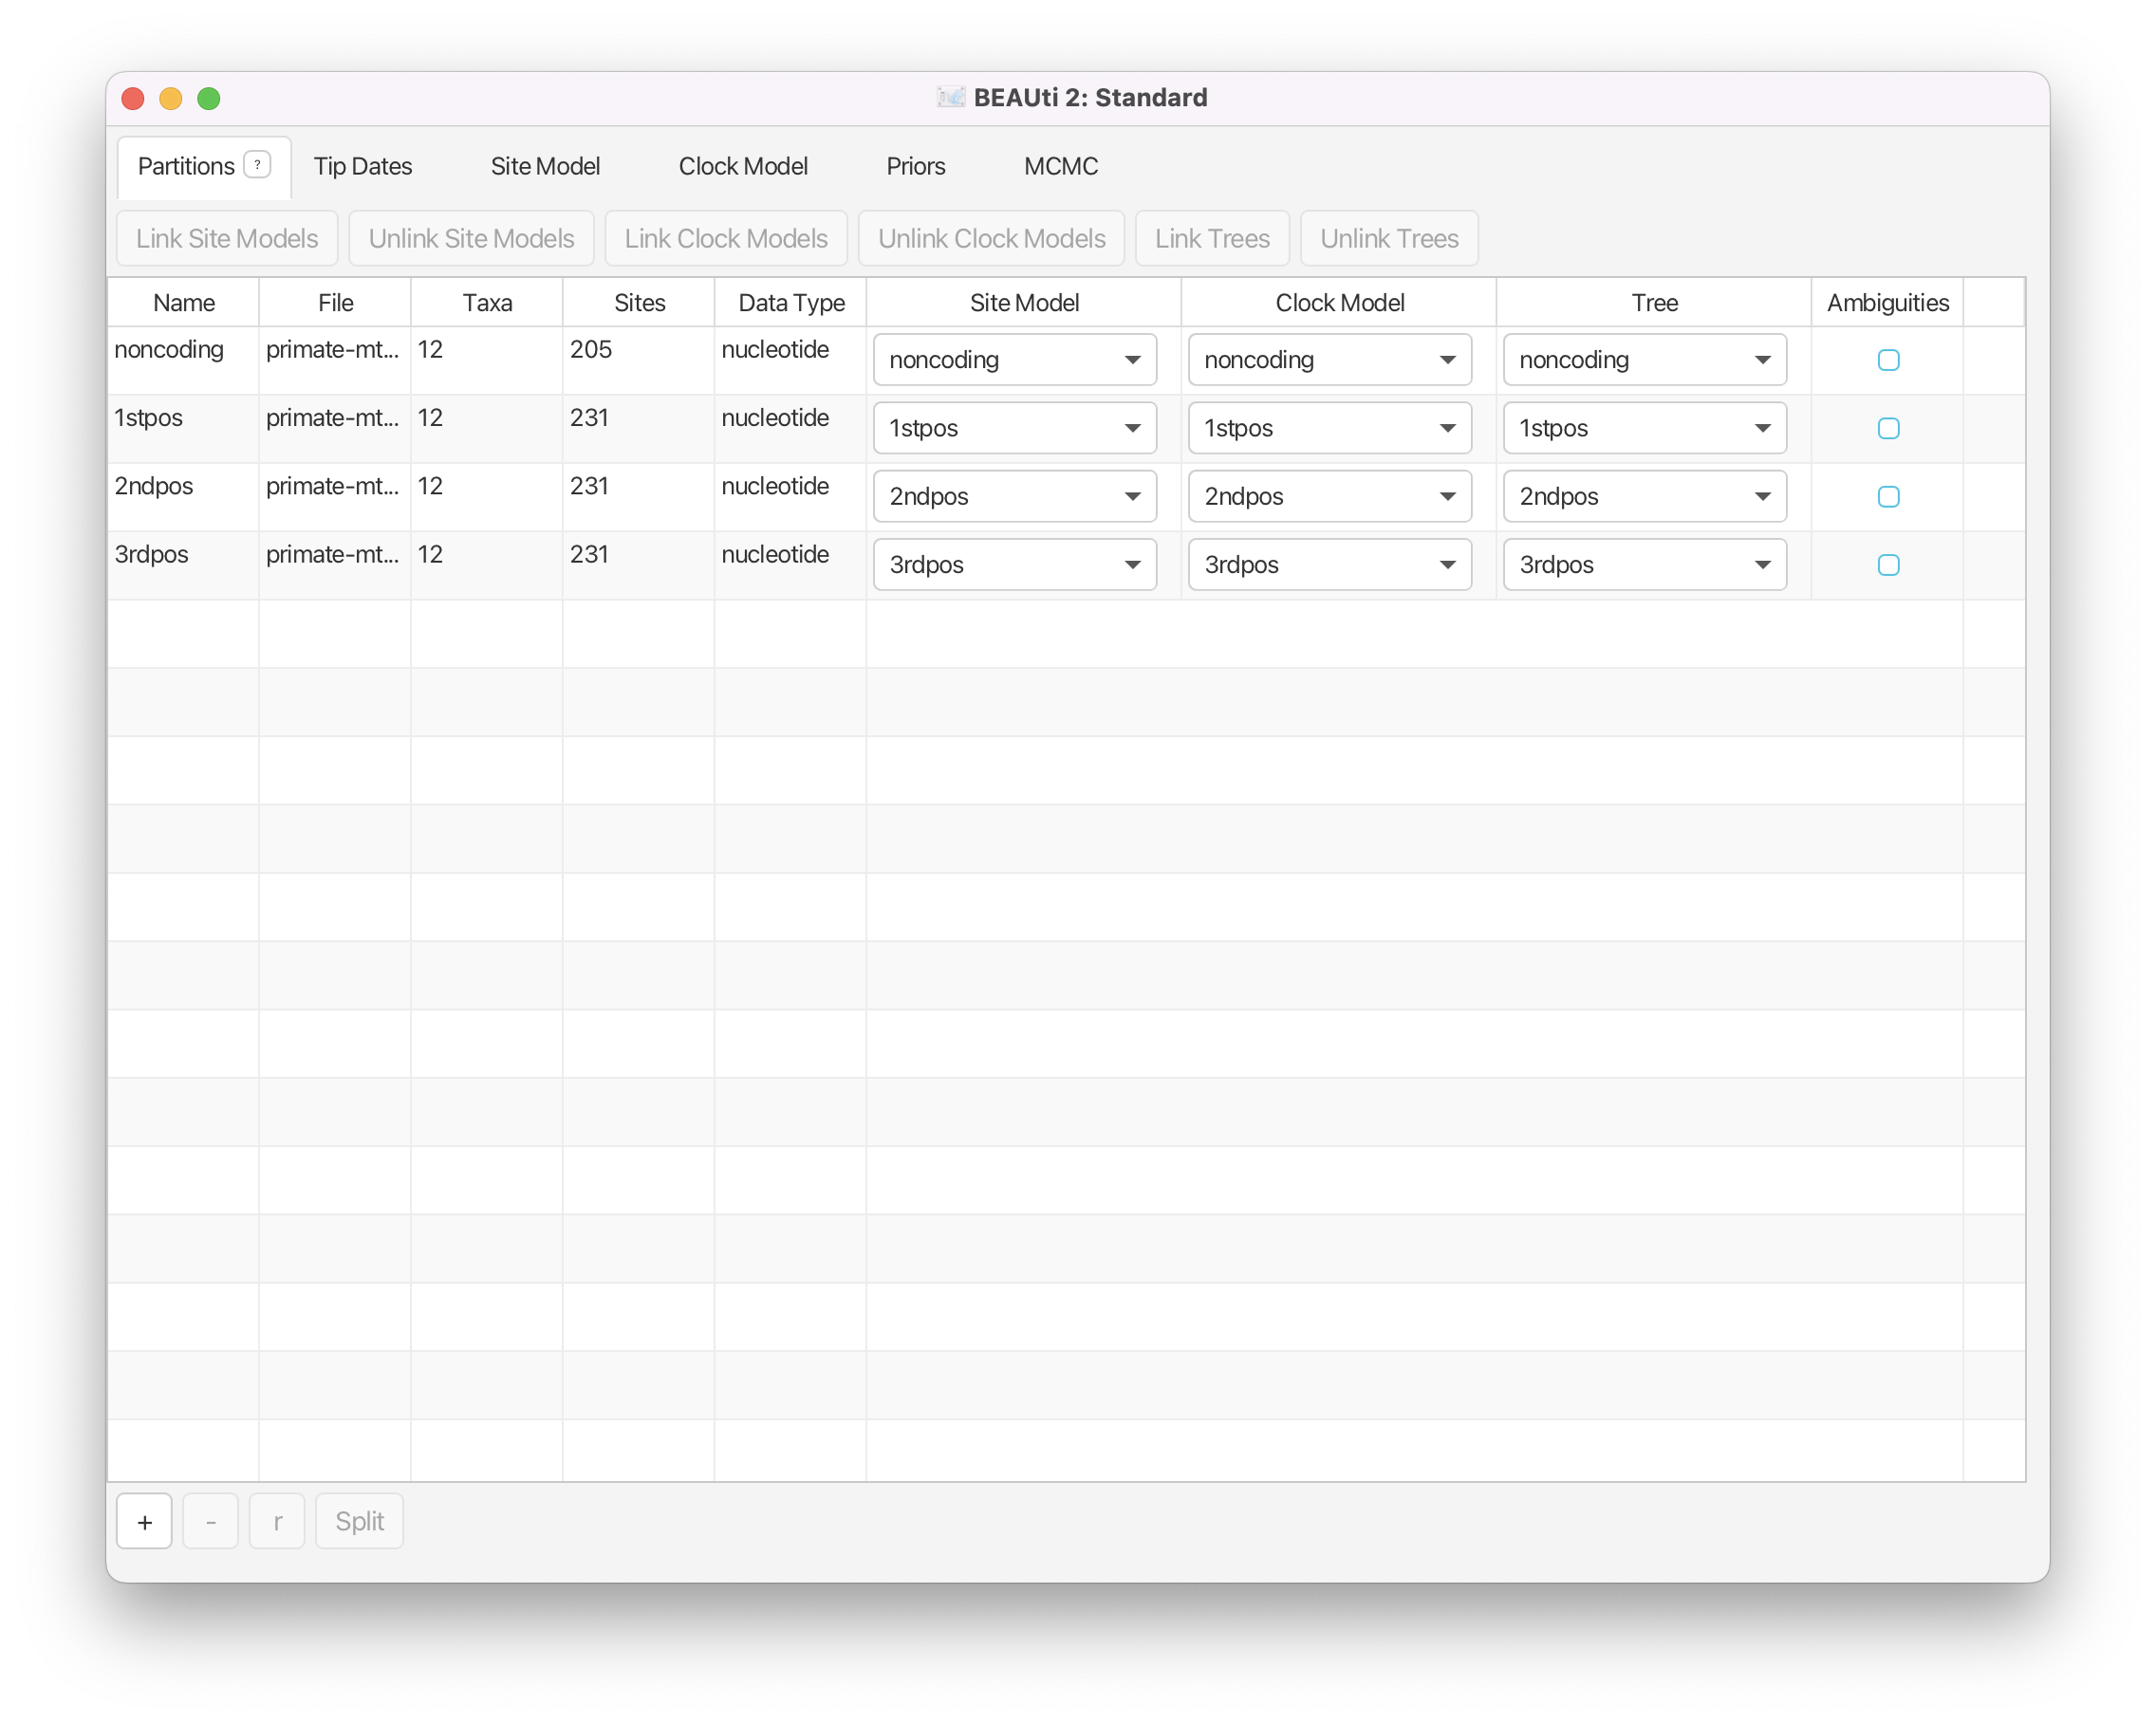
\includegraphics[max width=\textwidth, max height=0.9\textheight]{figures/data.png}
    \caption{Data imported into BEAUti2.}
    \label{fig:data}
\end{figure}

\hypertarget{setting-up-shared-models}{%
\subsubsection{Setting up shared
models}\label{setting-up-shared-models}}

A common way to account for site-to-site rate heterogeneity (variation
in substitution rates between different sites) is to use a Gamma site
model. In this model, one assumes that rate variation follows a Gamma
distribution. To make the analysis tractable the Gamma distribution is
discretised to a small number of bins (4-6 usually). The mean of each
bin then acts as a multiplier for the overall substitution rate. The
transition probabilities are then calculated for each scaled
substitution rate. To calculate the likelihood for a site,
\textbf{P(data \textbar{} tree, substitution model)} is calculated under
each Gamma rate category and the results are summed up to average over
all possible rates. This is a handy approach if one suspects that some
sites are mutating faster than others but the precise position of these
sites in the alignment is unknown or random.

Another way to account for site-to-site rate heterogeneity is to split
the alignment into explicit partitions, and specify an independent
substitution model for each partition. This is especially relevant when
one knows exactly which positions in the alignment are expected to
evolve at different rates. In our example, we split the alignment into
coding and non-coding regions, and further split the coding region into
1st, 2nd and 3rd codon positions. This information is encoded as
metadata into the \passthrough{\lstinline!.nex!} file, which BEAUti
automatically processes to produce the four partitions in the
\textbf{Partitions} tab as shown in Figure \ref{fig:data}.

\begin{framed}
\textbf{Double-click} on the different partitions (under the
\textbf{File} column) to view the individual alignments.
\end{framed}

\begin{figure}
    \centering
    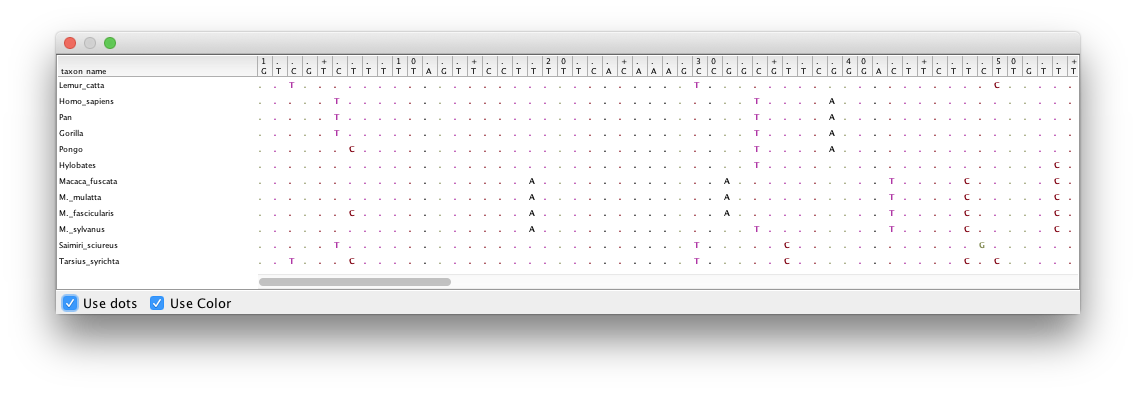
\includegraphics[max width=\textwidth, max height=0.9\textheight]{figures/2ndpos.png}
    \caption{The partition for the 2nd codon positions in the coding region of the primate mtDNA alignment.}
    \label{fig:2ndpos}
\end{figure}

\begin{figure}
    \centering
    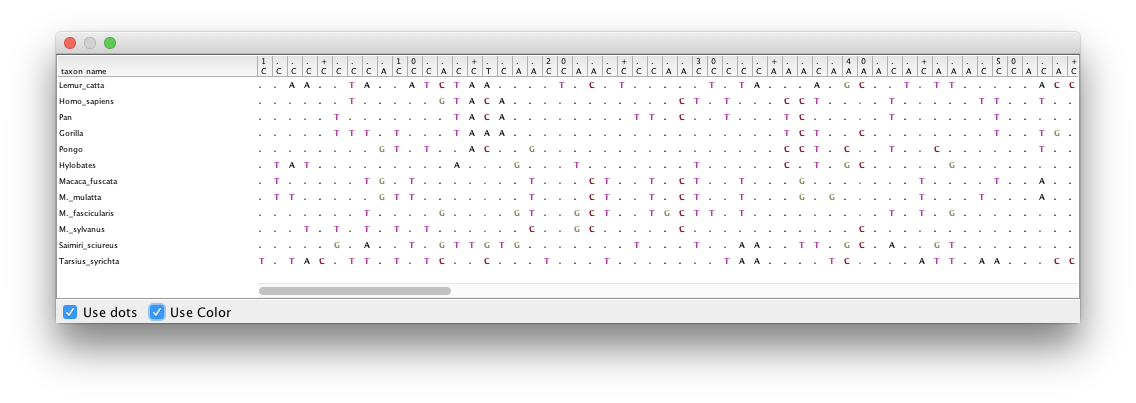
\includegraphics[max width=\textwidth, max height=0.9\textheight]{figures/3rdpos.png}
    \caption{The partition for the 3rd codon positions in the coding region of the primate mtDNA alignment.}
    \label{fig:3rdpos}
\end{figure}

By looking at the alignments for the 2nd and 3rd codon positions (Figure
\ref{fig:2ndpos} and Figure \ref{fig:3rdpos}) we can immediately see a
clear difference between the two codon positions. For the 2nd codon
position many of the ancestral relationships are clear from shared
substitutions between groups, for instance between the great apes
(\emph{Homo sapiens}, \emph{Pan}, \emph{Gorilla} and \emph{Pongo} -
humans, chimpanzees, gorillas and orangutans) and between the old-world
monkeys (\emph{Macaca fuscata}, \emph{M. mulatta}, \emph{M.
fascicularis} and \emph{M. sylvanus} - the macaques). The lesser apes
(represented by \emph{Hylobates} - gibbons) share most substitutions
with the great apes, but occasionally share a substitution with the
macaques. For the 3rd codon position there are many more substitutions
and the groupings are not as clear.

\begin{framed}
\textbf{Topic for discussion:} Do you think there is a good case for
using independent substitution models on the different partitions in the
\passthrough{\lstinline!.nex!} file? Do you think this is sufficient for
taking all site-to-site rate variation into account?

How would you account for rate variation between sites \emph{within}
each partition?
\end{framed}

Since all of the sequences in this dataset are from the mitochondrial
genome (which is not believed to undergo recombination in birds and
mammals) they all share the same ancestry. By default, BEAST2 would
recover a separate, independent time-calibrated tree for each partition,
so we need to make sure that it uses all data to recover only a single
shared tree. For the sake of simplicity, we will also assume that the
partitions have the same evolutionary branch-rate distribution, and
hence share the clock model as well.

To make sure that the partitions share the same evolutionary history we
need to link the \textbf{clock model} and the \textbf{tree} in BEAUti.

\begin{framed}
Select all four data partitions the \textbf{Partitions} panel (use
\textbf{shift+click}) and click the \textbf{Link Trees} and \textbf{Link
Clock Models} buttons.
\end{framed}

You will see that the \textbf{Clock Model} and the \textbf{Tree} columns
in the table both changed to say \passthrough{\lstinline!noncoding!}.
Now we will rename both models such that the following options and
generated log files are easier to read. The resulting setup should look
as shown in Figure \ref{fig:link}.

\begin{framed}
Click on the first drop-down menu in the \textbf{Clock Model} column and
rename the shared clock model to \passthrough{\lstinline!clock!}.

Likewise, rename the shared tree to \passthrough{\lstinline!tree!}.
\end{framed}

\begin{figure}
    \centering
    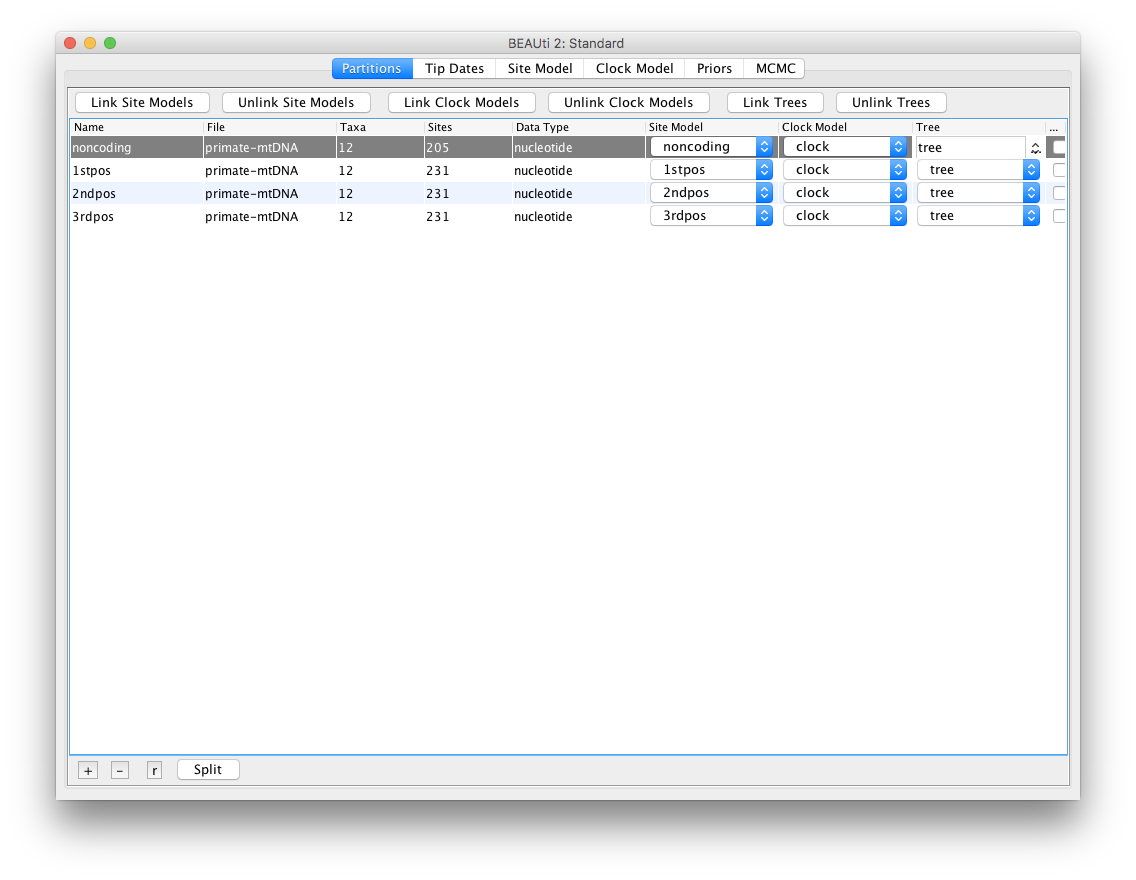
\includegraphics[max width=\textwidth, max height=0.9\textheight]{figures/link.png}
    \caption{Linked clock and tree models.}
    \label{fig:link}
\end{figure}

\hypertarget{setting-the-substitution-model}{%
\subsubsection{Setting the substitution
model}\label{setting-the-substitution-model}}

In this analysis all of our sequences come from extant species and were
thus all sampled in the present day (assumed to be
\passthrough{$ t = 0 $}). Therefore we do not need to set
sampling dates and we skip the \textbf{Tip Dates} panel. Next, we need
to set the substitution model in the \textbf{Site Model} tab.

\begin{framed}
Select the \textbf{Site Model} tab.
\end{framed}

The options available in this panel depend on whether the alignment data
are in nucleotides, amino-acids, binary data or general data. The
settings available after loading the alignment will contain the default
values we normally want to modify.

The panel on the left shows each partition. Remember that we did not
link the substitution models in the previous step for the different
partitions, so each partition evolves under a different substitution
model, i.e.~we assume that different positions in the alignment
accumulate substitutions differently. We will need to set the site model
separately for each part of the alignment as these models are unlinked.
However, we think that all partitions evolve according to the same
general model (albeit with different parameter values).

\begin{framed}
Make sure that \passthrough{\lstinline!noncoding!} is selected.

\begin{itemize}

\item
  Check the \textbf{estimate} checkbox for \textbf{Substitution Rate}.
\item
  Set the \textbf{Gamma Category Count} to 4.
\item
  Check the \textbf{estimate} box for the \textbf{Shape} parameter (it
  should already be checked).
\item
  Select \textbf{HKY} in the \textbf{Subst Model} drop-down menu.
\item
  Ensure that the \textbf{estimate} box for \textbf{Kappa} is checked
  (it should already be checked).
\item
  Select \textbf{Empirical} from the \textbf{Frequencies} drop-down
  menu.
\end{itemize}

Note that when you checked \textbf{estimate} for the substitution rate
the greyed out \textbf{Fix mean substitution rate} box at the bottom of
the window was also automatically checked.
\end{framed}

\begin{figure}
    \centering
    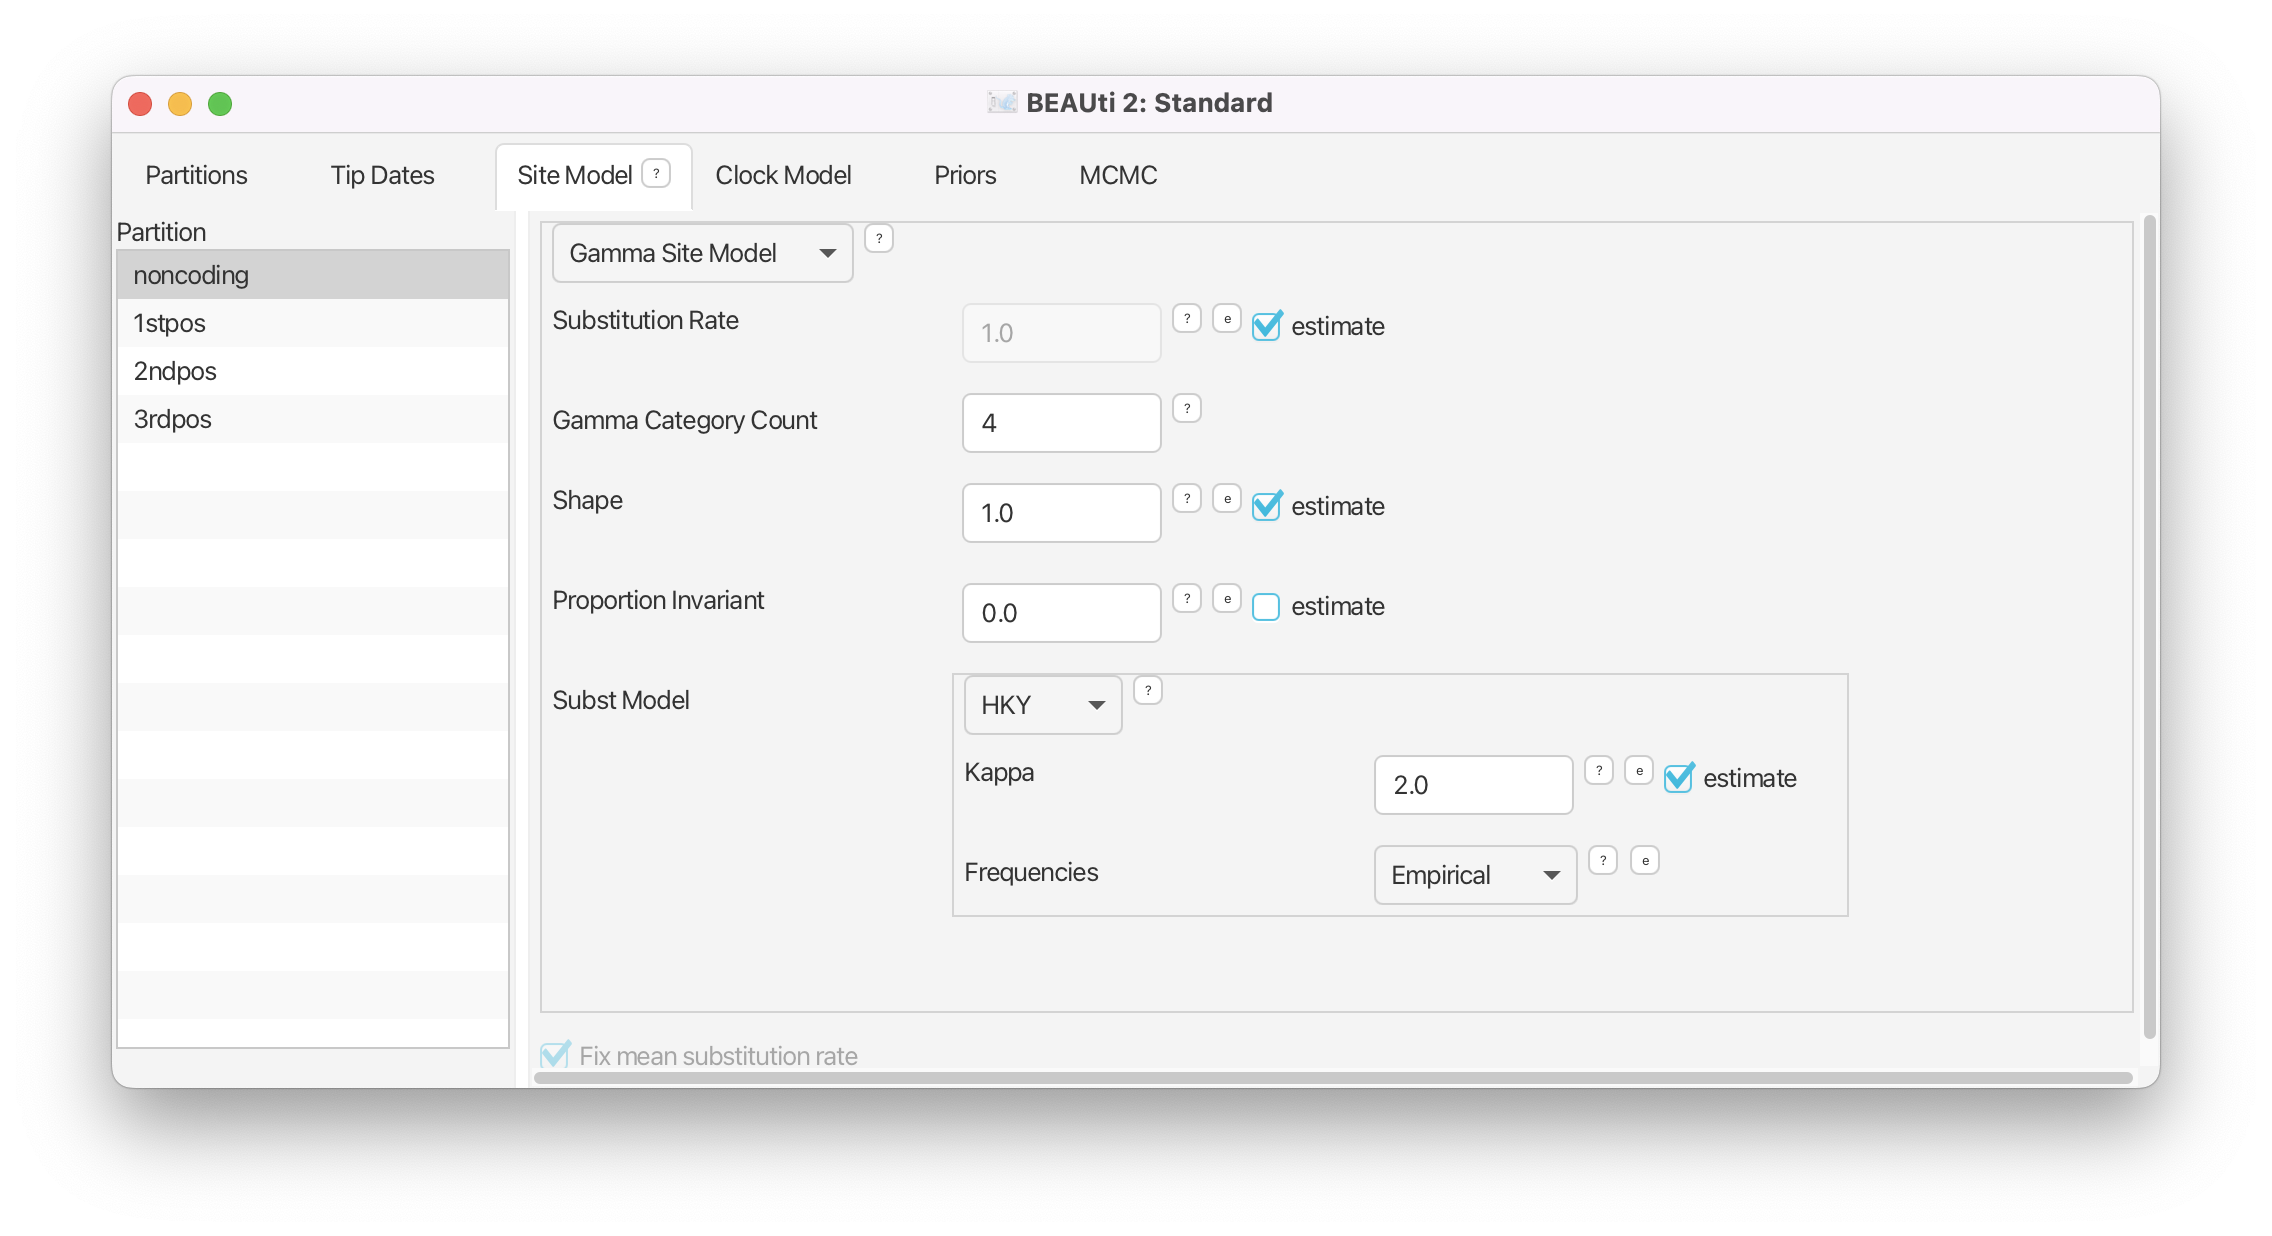
\includegraphics[max width=\textwidth, max height=0.9\textheight]{figures/substitution.png}
    \caption{Site model setup.}
    \label{fig:subst}
\end{figure}

The panel should now look like Figure \ref{fig:subst}.

We are using an HKY substitution model with empirical frequencies. This
will fix the frequencies to the proportions observed in the partition.
This approach means that we can get a good fit to the data without
explicitly estimating these parameters. To model site-to-site rate
variation within each partition we use a discrete Gamma site model with
4 categories. Now we \emph{could} repeat the above steps for each of the
remaining partitions or we can take a shortcut.

\begin{framed}
Select the remaining three partitions (use \textbf{shift+click}). The
window will now look like Figure \ref{fig:clone}.

Select \passthrough{\lstinline!noncoding!} and click \textbf{OK} to to
clone the site model for the other three partitions from
\passthrough{\lstinline!noncoding!}.
\end{framed}

\begin{figure}
    \centering
    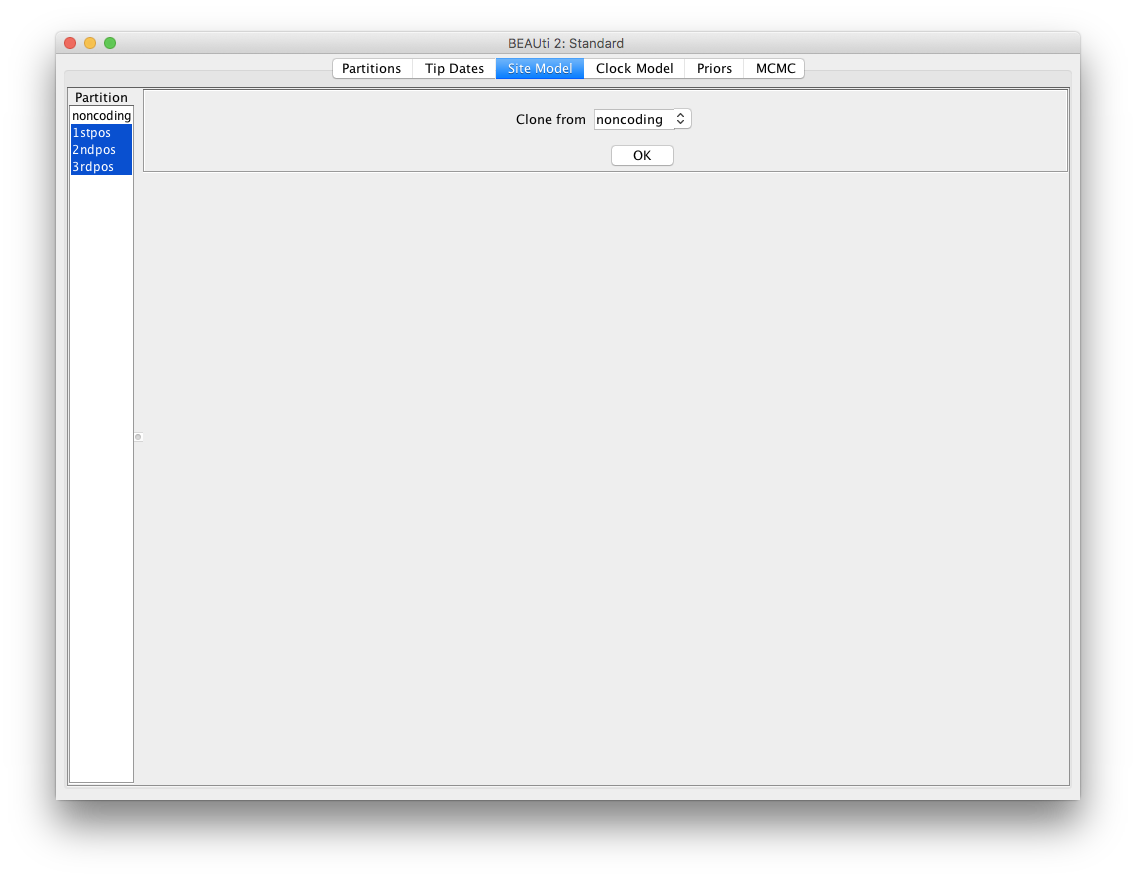
\includegraphics[max width=\textwidth, max height=0.9\textheight]{figures/clone.png}
    \caption{Shortcut to clone site models between partitions.}
    \label{fig:clone}
\end{figure}

\begin{framed}
\textbf{Topic for discussion:} Can you figure out the reason why
\textbf{Fix mean substitution rate} was automatically checked when you
checked \textbf{estimate} for the substitution rate? Don't worry if you
can't figure it out, it is explained in detail in later tutorials.
\end{framed}

\hypertarget{setting-the-clock-model}{%
\subsubsection{Setting the clock model}\label{setting-the-clock-model}}

Next, select the \textbf{Clock Model} tab at the top of the main window.
This is where we set up the molecular clock model. For this exercise we
are going to leave the selection at the default value of a strict
molecular clock, because this data is very clock-like and does not need
rate variation among branches to be included in the model.

\begin{framed}
Click on the \textbf{Clock Models} tab and view the setup \emph{(but
don't do anything)}.
\end{framed}

Note that the \textbf{estimate} box next to \textbf{Mean clock rate} is
not checked.

\hypertarget{setting-priors}{%
\subsubsection{Setting priors}\label{setting-priors}}

The \textbf{Priors} tab allows prior distributions to be specified for
each model parameter. The model selections made in the \textbf{Site
Model} and \textbf{Clock Model} tabs determine which parameters are
included in the model. For each of these parameters a prior distribution
needs to be specified. It is also possible to specify hyperpriors (and
hyper-hyperpriors etc.) for each of the model parameters. We also need
to specify a prior for the \textbf{Tree}. In this example the tree prior
is a null model for species diversity over time within the primates.

Here we specify that we wish to use the Calibrated Yule model as the
tree prior. This is a simple model of speciation that is generally
appropriate when considering sequences from different species.

\begin{framed}
Go to the \textbf{Priors} tab and select \textbf{Calibrated Yule Model}
in the drop-down menu next to \textbf{Tree.t:tree}.
\end{framed}

The \textbf{birthRate} parameter measures the rate of speciation in the
calibrated Yule model. We will set an unspecific Gamma prior for this
parameter.

\begin{framed}
For \textbf{birthRateY.t:tree} select \textbf{Gamma} from the drop-down
menu

\begin{itemize}

\item
  Expand the options for \textbf{birthRateY.t:tree} using the arrow
  button on the left.
\item
  Set the \textbf{Alpha} (shape) parameter to \textbf{0.001} and the
  \textbf{Beta} (scale) parameter to \textbf{1000}.
\end{itemize}
\end{framed}

Note that BEAUti displays a plot of the prior distribution on the right,
as well as a few of its quantiles. This is for easy reference and can
help us to decide if a prior is appropriate. The unspecific Gamma prior
we are using is defined on \passthrough{$ (0,\infty) $} and
has a very broad range of values included between its 2.5\% and 97.5\%
quantiles.

If we wanted to add a hyperprior on one of the parameters of the Gamma
prior we would check the \textbf{estimate} box on the right of the
parameter. We could also change the initial values or limits of the
model parameters by clicking on the boxes next to the drop-down menus.
Do \textbf{not} do this here, as we are \textbf{not} adding any
hyperpriors or changing limits in this analysis!

\textbf{We will leave the rest of the priors on their default values!}
The BEAUti panel should look as shown in Figure \ref{fig:priors}.

Please note that in general using default priors is frowned upon as
priors are meant to convey your prior knowledge of the parameters. It is
important to know what information the priors add to the MCMC analysis
and whether this fits your particular situation. In our case the default
priors are suitable for this particular analysis, however for further,
more complex analyses, we will require a clear idea of what the priors
mean. Getting this understanding is difficult and comes with experience.
The topic of choosing priors is discussed in more detail in later
tutorials.

\begin{figure}
    \centering
    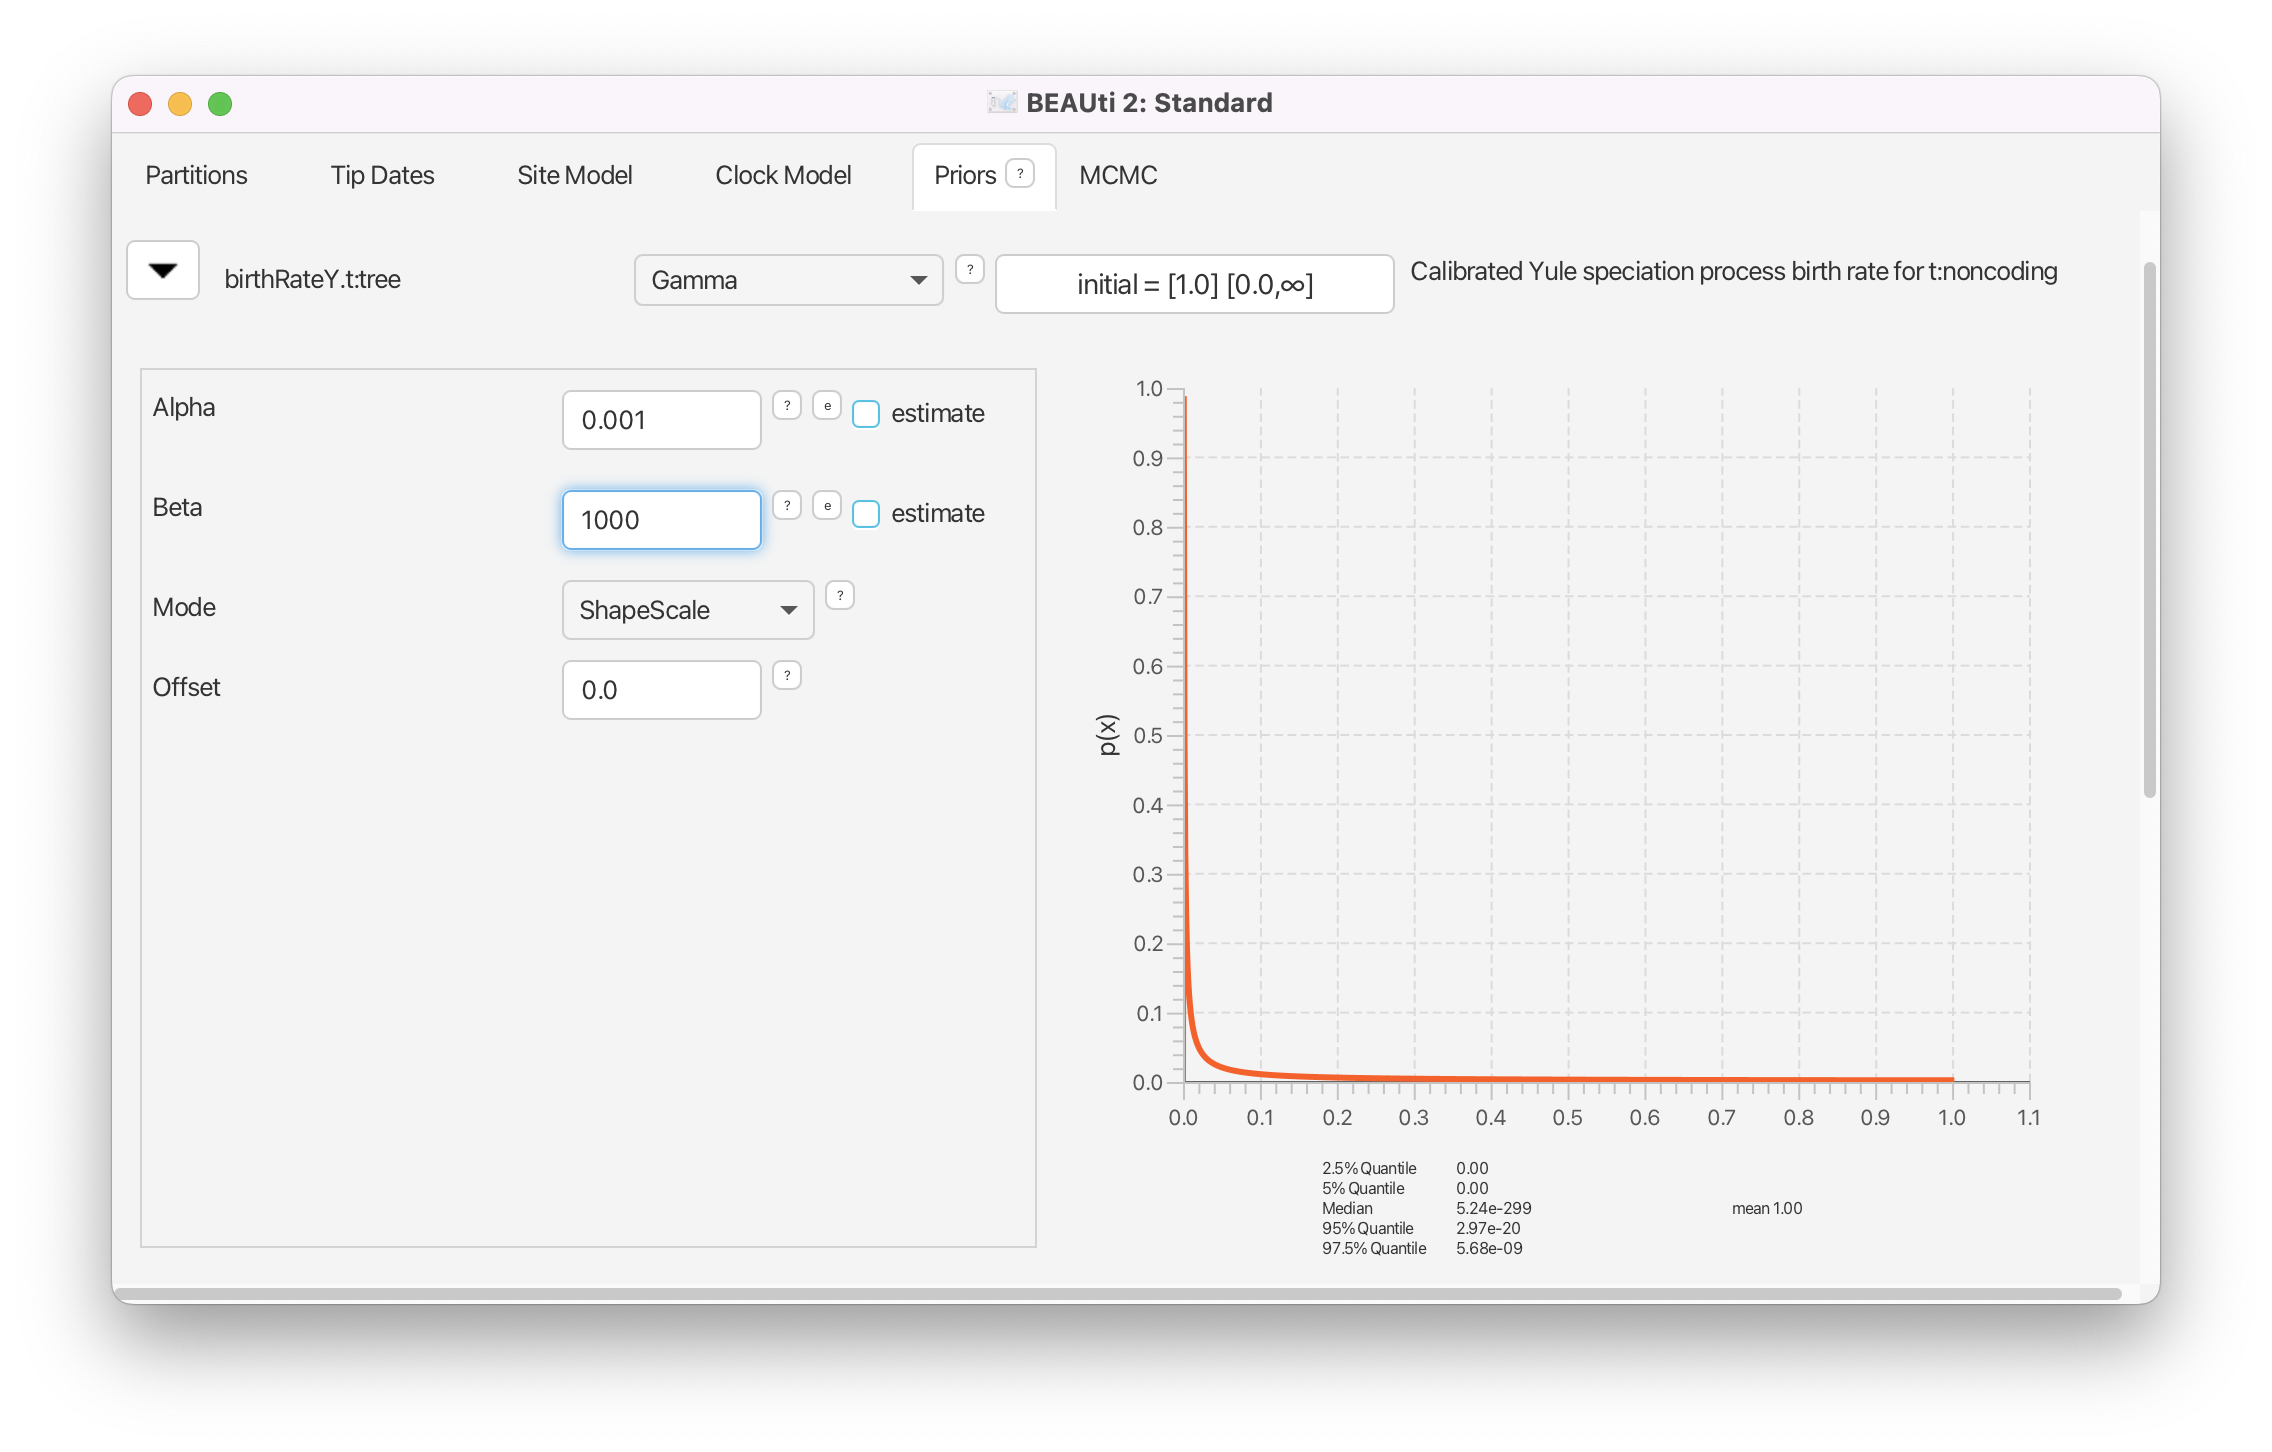
\includegraphics[max width=\textwidth, max height=0.9\textheight]{figures/priors.png}
    \caption{Prior setup.}
    \label{fig:priors}
\end{figure}

\hypertarget{adding-a-calibration-node}{%
\subsubsection{Adding a calibration
node}\label{adding-a-calibration-node}}

Since all of the samples come from a single time point, there is no
information on the actual height of the phylogenetic tree in time units.
That means the tree height (tMRCA) and substitution rate parameters will
not be distinguishable and BEAST2 will only be able to estimate their
product. To allow BEAST2 to separate these two parameters we need to
input additional information that will help calibrate the tree in time.

In a Bayesian analysis, additional information from external sources
should be encoded in the form of a prior distribution. Thus, we will
have to add a new prior to the model.

\begin{framed}
To add an extra prior to the model, press the \textbf{+ Add Prior}
button below the list of priors. If this doesn't automatically open a
\textbf{Taxon set editor} window, select \textbf{MRCA Prior} from the
drop-down menu.

You will see a dialogue box (\textbf{Taxon set editor}) that allows you
to select a subset of taxa from the phylogenetic tree. Once you have
created a taxon set you will be able to add calibration information for
its most recent common ancestor (MRCA) later on.

\begin{itemize}

\item
  Set the \textbf{Taxon set label} to
  \passthrough{\lstinline!human-chimp!}.
\item
  Locate \passthrough{\lstinline!Homo\_sapiens!} in the left hand side
  list and click the \textbf{\textgreater\textgreater{}} button to add
  it to the \passthrough{\lstinline!human-chimp!} taxon set.
\item
  Locate \passthrough{\lstinline!Pan!} in the left hand side list and
  click the \textbf{\textgreater\textgreater{}} button to add it to the
  \passthrough{\lstinline!human-chimp!} taxon set.
\end{itemize}
\end{framed}

The taxon set should now look like Figure \ref{fig:taxa}.

\begin{framed}
Click the \textbf{OK} button to add the newly defined taxon set to the
prior list.
\end{framed}

\begin{figure}
    \centering
    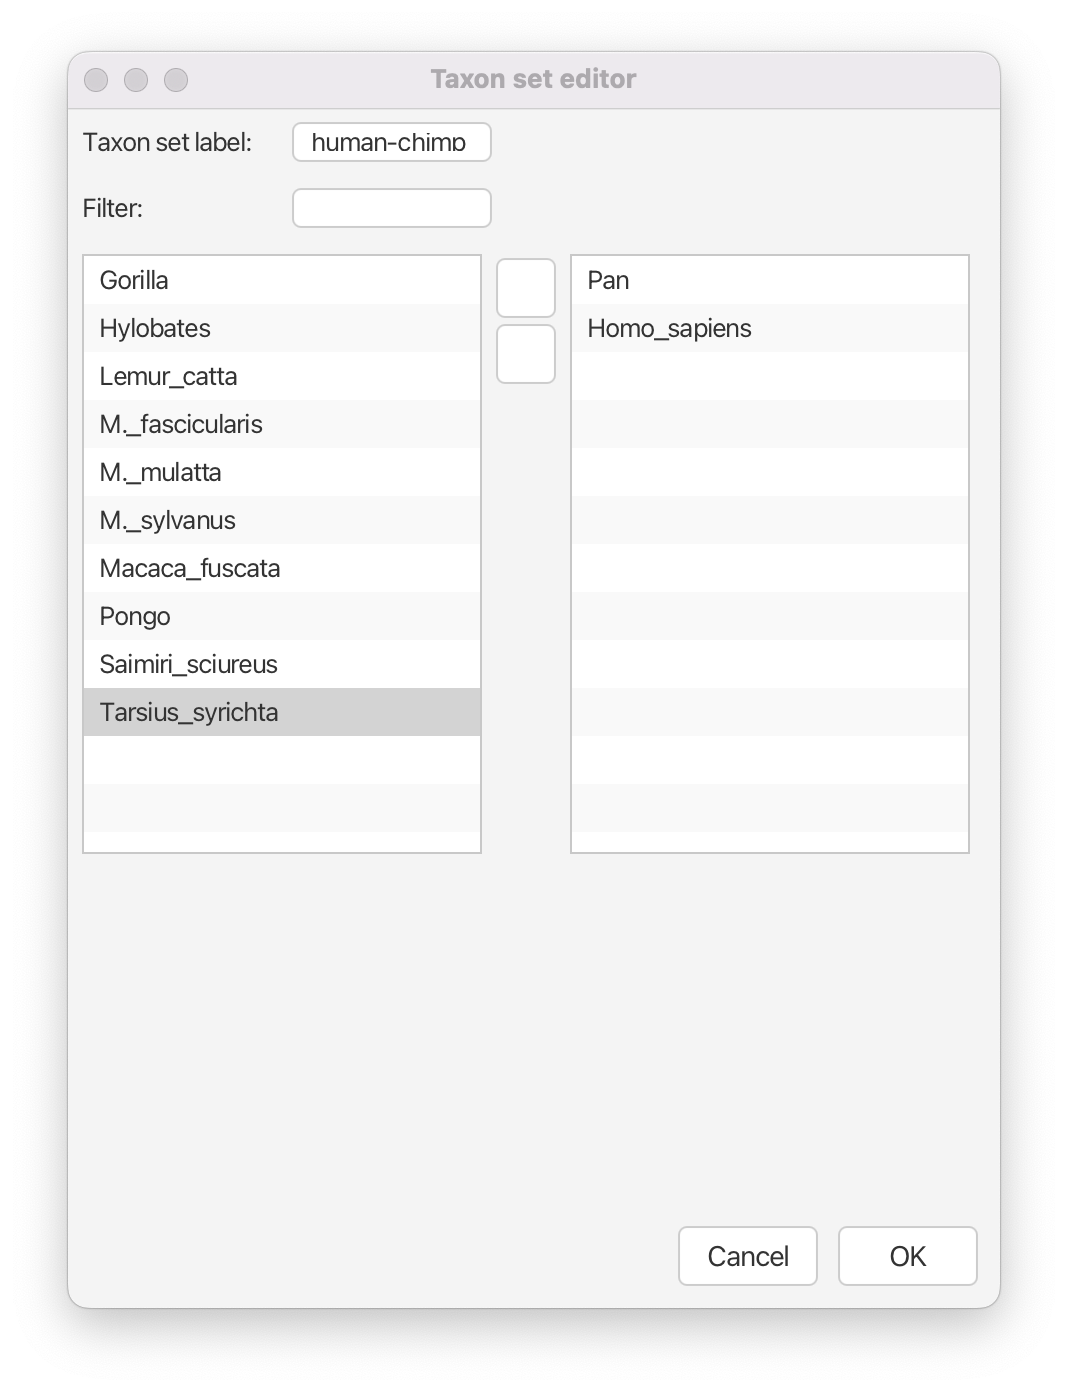
\includegraphics[width=0.600000\textwidth]{figures/taxa.png}
    \caption{Calibration node taxon set.}
    \label{fig:taxa}
\end{figure}

The new node we have added is a calibrated node on the human-chimpanzee
split to be used in conjunction with the Calibrated Yule prior. In order
for that to work we need to enforce monophyly. This will constrain the
tree topology so that the human-chimp grouping is kept monophyletic
during the course of the MCMC analysis.

\begin{framed}
Check the \textbf{monophyletic} checkbox next to the
\textbf{human-chimp.prior}.
\end{framed}

We now need to specify a prior distribution on the calibration node
based on our prior knowledge from fossils in order to calibrate our
tree. We will use a Normal distribution with mean 6 MYA and a standard
deviation of 0.5 million years. This will give a central 95\% range of
about 5-7 million years, which roughly corresponds to the current
consensus estimate of the date of the most recent common ancestor of
humans and chimpanzees.

\begin{framed}
Select \textbf{Normal} from the drop-down menu to the right of the newly
added \textbf{human-chimp.prior}.

\begin{itemize}

\item
  Expand the distribution options using the arrow button on the left.
\item
  Set the \textbf{Mean} of the distribution to \textbf{6}.
\item
  Set the \textbf{Sigma} of the distribution to \textbf{0.5}.
\end{itemize}
\end{framed}

The final setup of the calibration node prior should look as shown in
Figure \ref{fig:calibration}.

\begin{figure}
    \centering
    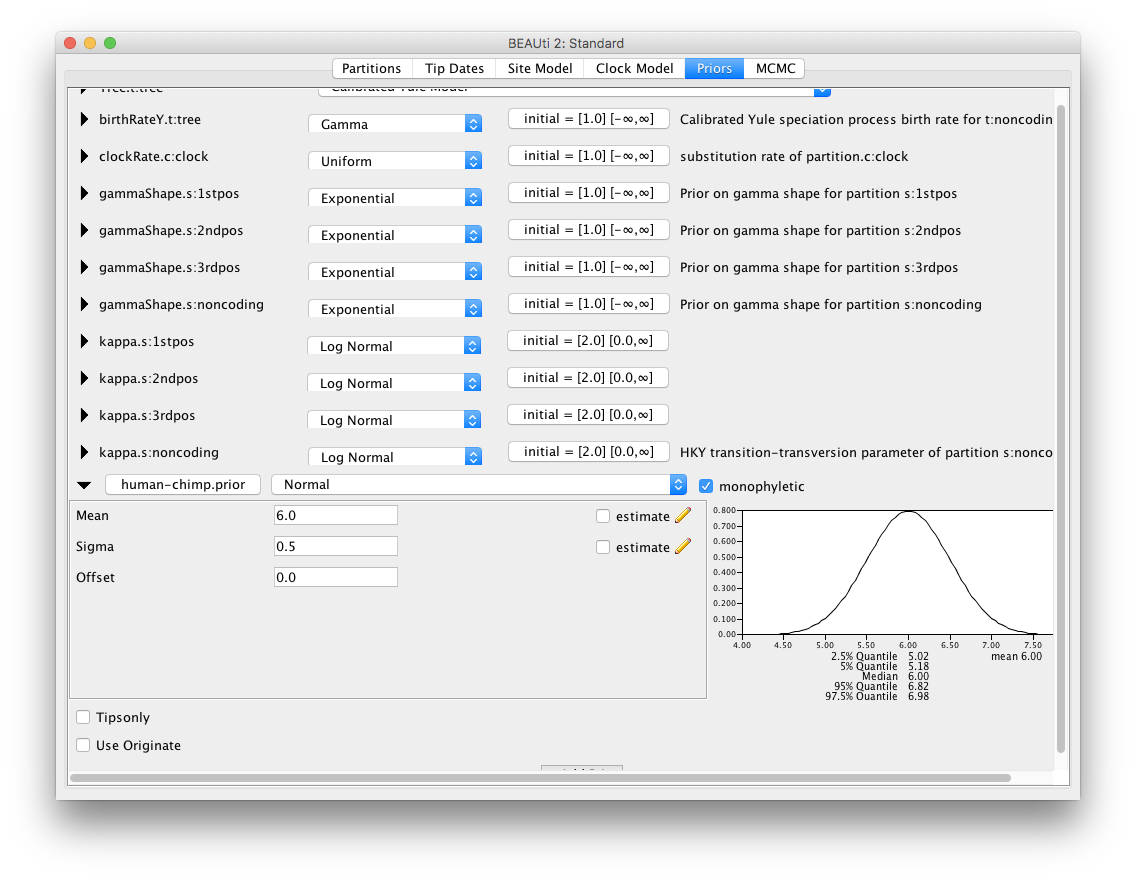
\includegraphics[max width=\textwidth, max height=0.9\textheight]{figures/calibration.png}
    \caption{Calibration node prior setup.}
    \label{fig:calibration}
\end{figure}

\begin{framed}
\textbf{Topic for discussion:} After setting the calibration node prior
a new prior for \passthrough{\lstinline!clockrate.c:clock!} magically
appeared in the priors tab! If you go back to the \textbf{Clock model}
tab you'll see that the \textbf{estimate} box next to \textbf{Mean clock
rate} is now checked and greyed out (cannot be unchecked).

What just happened?
\end{framed}

\hypertarget{setting-the-mcmc-options}{%
\subsubsection{Setting the MCMC
options}\label{setting-the-mcmc-options}}

Finally, the \textbf{MCMC} tab allows us to control the length of the
MCMC chain and the frequency of stored samples. It also allows one to
change the output file names.

\begin{framed}
Go to the \textbf{MCMC} tab.
\end{framed}

The \textbf{Chain Length} parameter specifies the number of steps the
MCMC chain will make before finishing (i.e.~the number of accepted
proposals). This number depends on the size of the dataset, the
complexity of the model and the precision of the answer required. The
default value of 10'000'000 is arbitrary and should be adjusted
accordingly. For this small dataset we initially set the chain length to
1'000'000 such that this analysis will take only a few minutes on most
modern computers (rather than hours). We leave the \textbf{Store Every}
and \textbf{Pre Burnin} fields at their default values.

\begin{framed}
Set the \textbf{Chain Length} to 1'000'000.
\end{framed}

Below these general settings you will find the logging settings. Each
particular option can be viewed in detail by clicking the arrow to the
left of it. You can control the names of the log files and how often
values will be stored in each of the files.

Start by expanding the \textbf{tracelog} options. This is the log file
you will use later to analyse and summarise the results of the run. The
\textbf{Log Every} parameter for the log file should be set relative to
the total length of the chain. Sampling too often will result in very
large files with little extra benefit in terms of the accuracy of the
analysis. Sampling too sparsely will mean that the log file will not
record sufficient information about the distributions of the parameters.
We normally want to aim to store no more than 10'000 samples so this
should be set to no less than chain length/10'000. For this analysis we
will make BEAST2 write to the log file every 200 samples.

\begin{framed}
Expand the \textbf{tracelog} options.

\begin{itemize}

\item
  Set the \textbf{Log Every} parameter to \textbf{200}.
\item
  Leave the filename as is (\passthrough{\lstinline!$(filebase).log!}).
\end{itemize}
\end{framed}

Next, expand the \textbf{screenlog} options. The screen output is simply
for monitoring the program's progress. Since it is not so important,
especially if you run your analysis on a remote computer or a computer
cluster, the \textbf{Log Every} can be set to any value. However, if it
is set too small, the sheer quantity of information being displayed on
the screen will actually slow the program down. For this analysis we
will make BEAST2 log to screen every 1'000 samples, which is the default
setting.

\begin{framed}
Expand the \textbf{screenlog} options.

\begin{itemize}

\item
  Leave the \textbf{Log Every} parameter at the default value of 1'000.
\end{itemize}
\end{framed}

Finally, we can also change the tree logging frequency by expanding
\textbf{treelog.t:tree}. For big trees with many taxa each individual
tree will already be quite large, thus if you log lots of trees the tree
files can easily become extremely large. You will be amazed at how
quickly BEAST can fill up even the biggest of drives if the tree logging
frequency is too high! For this reason it is often a good idea to set
the tree logging frequency lower than the trace log (especially for
analyses with many taxa). However, be careful, as the post-processing
steps of some models (such as the Bayesian skyline plot) require the
trace and tree logging frequencies to be identical!

\begin{framed}
Expand the \textbf{treelog.t:tree} options.

\begin{itemize}

\item
  Set the \textbf{File Name} to
  \passthrough{\lstinline!primate-mtDNA.trees!}.
\item
  Leave the \textbf{Log Every} parameter at the default value of 1'000.
\end{itemize}
\end{framed}

The final setup should look as in Figure \ref{fig:logs}.

\begin{figure}
    \centering
    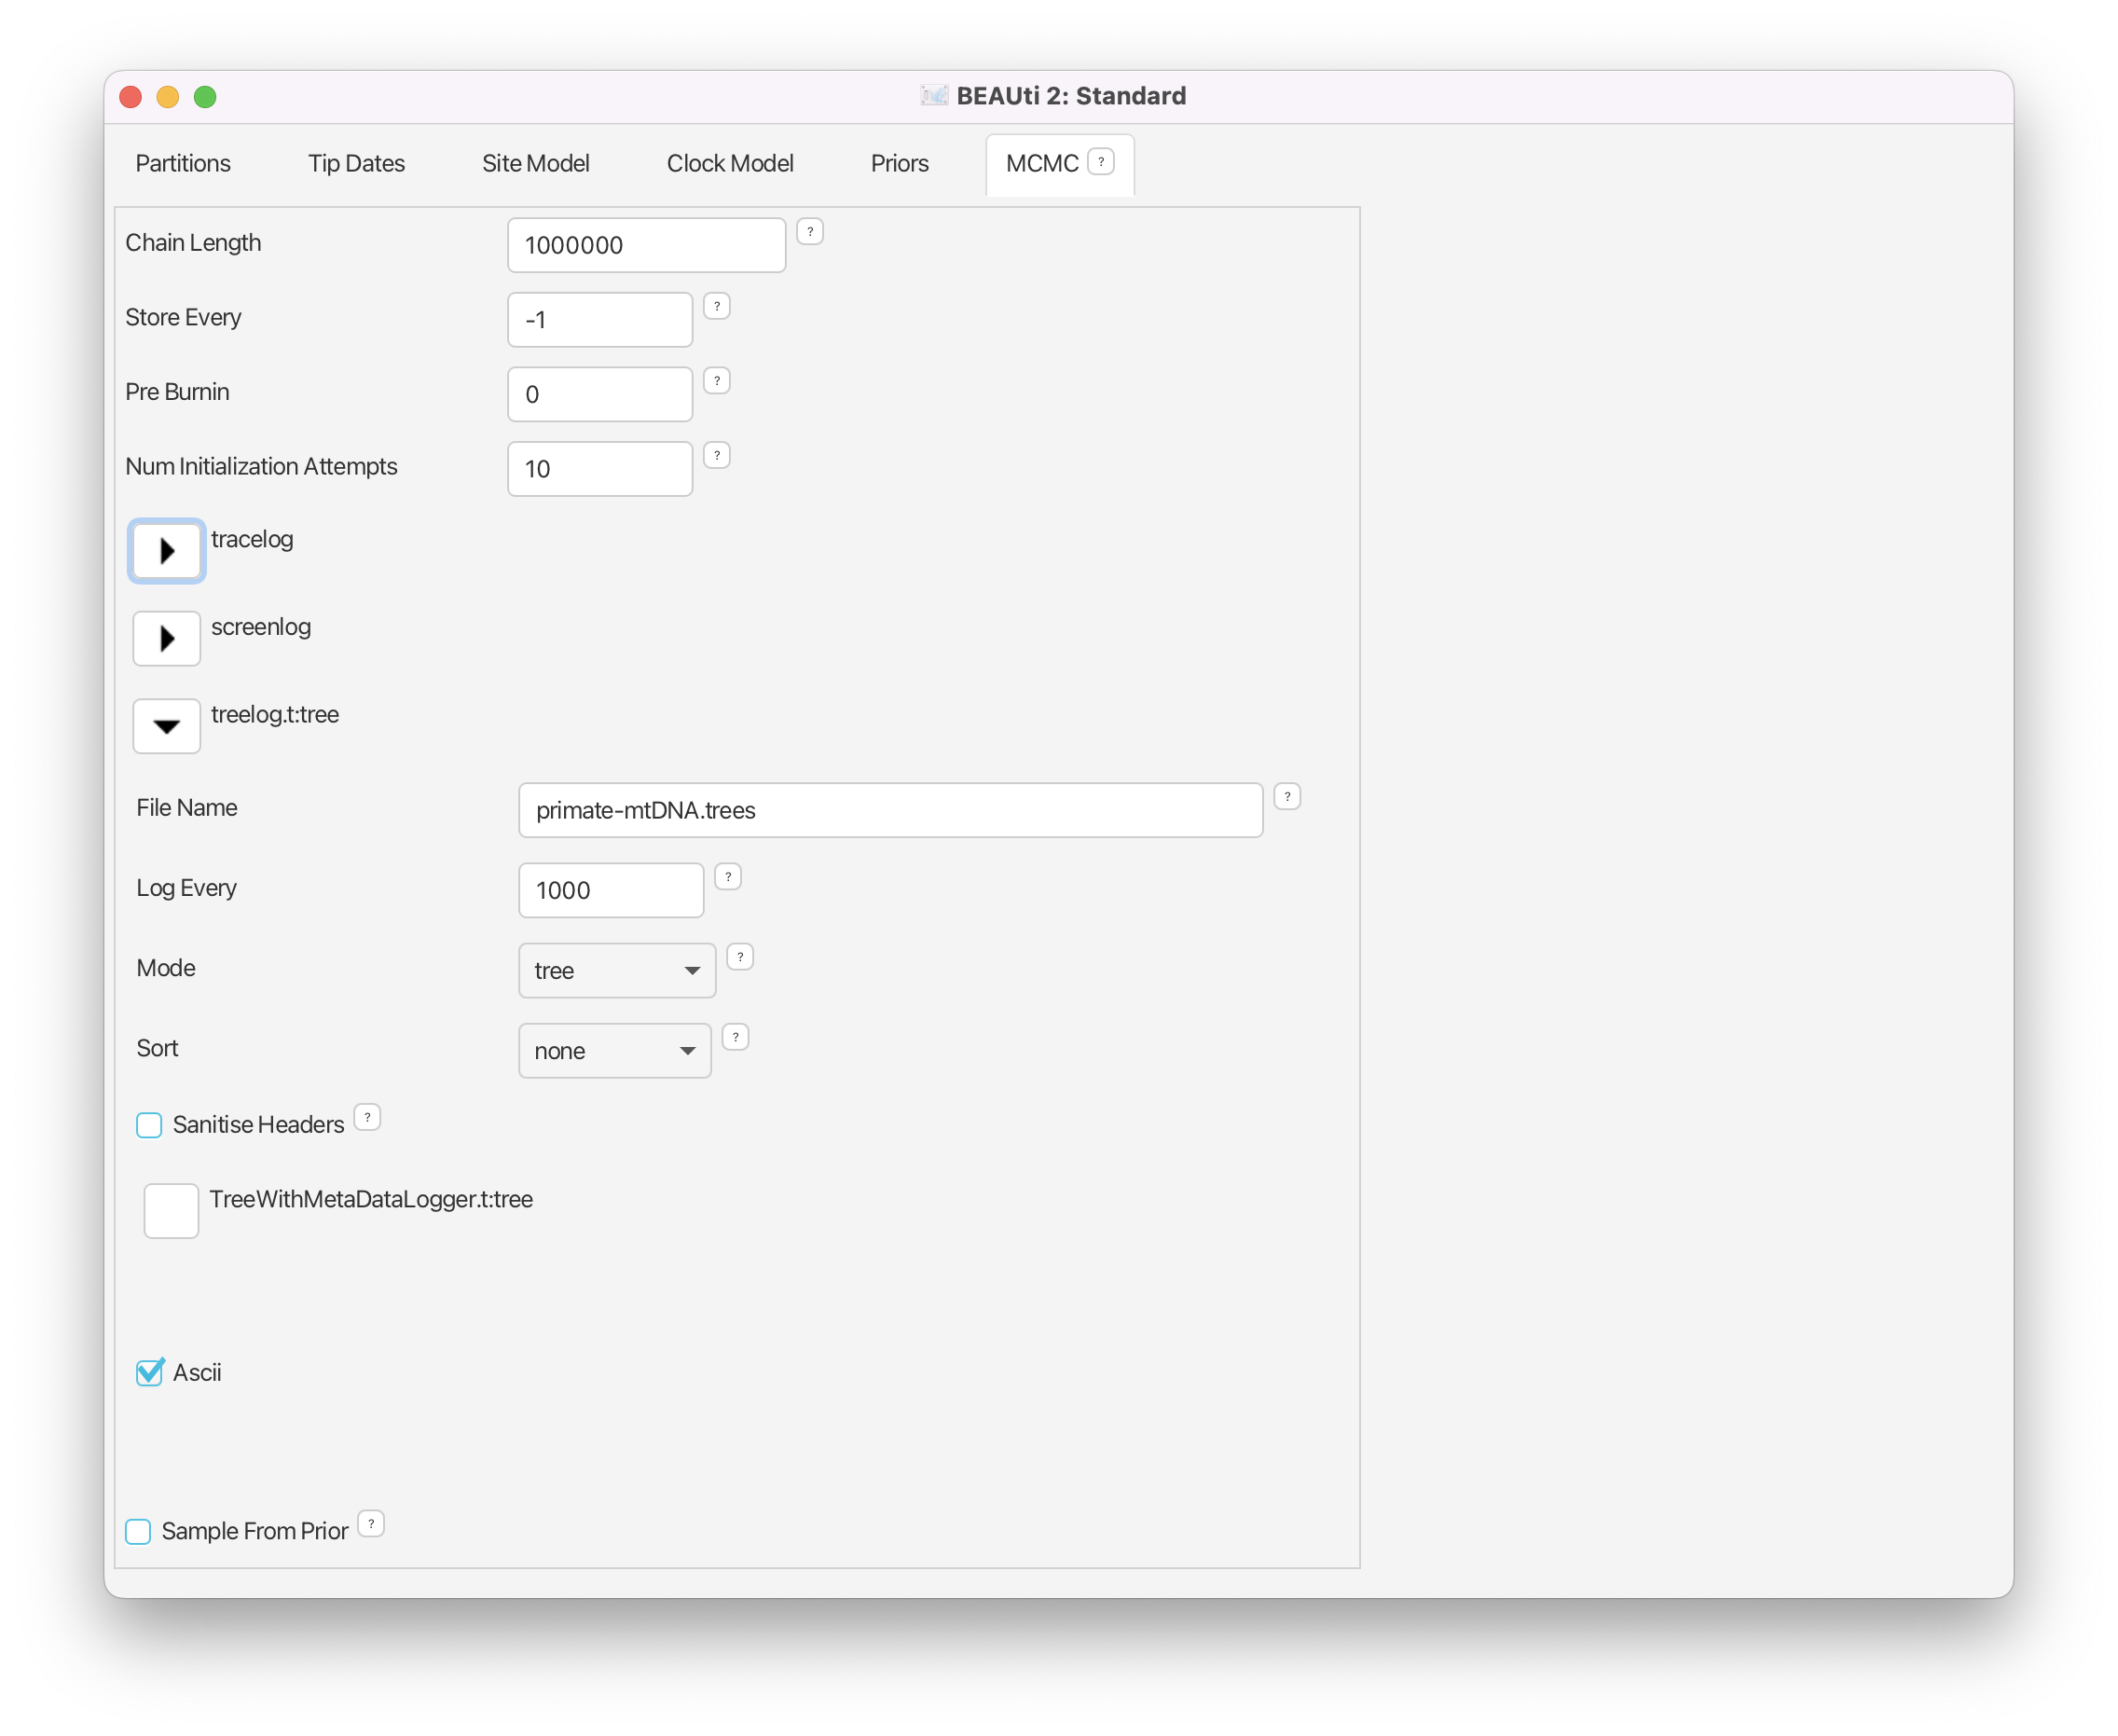
\includegraphics[max width=\textwidth, max height=0.9\textheight]{figures/logs.png}
    \caption{Logging options.}
    \label{fig:logs}
\end{figure}

\hypertarget{generating-the-xml-file}{%
\subsubsection{Generating the XML file}\label{generating-the-xml-file}}

We are now ready to create the BEAST2 XML file. This is the final
configuration file BEAST2 can use to execute the analysis.

\begin{framed}
Save the XML file under the name
\passthrough{\lstinline!primates-mtDNA.xml!} using \textbf{File
\textgreater{} Save}.
\end{framed}

\clearpage

\hypertarget{running-the-analysis}{%
\subsection{Running the analysis}\label{running-the-analysis}}

Now run BEAST2 and provide your newly created XML file as input. You can
also change the \textbf{random number seed} for the run. This number is
the starting point of a pseudo-random number chain BEAST2 will use to
generate the samples. As computers are unable to generate truly random
numbers, we have to resort to generating deterministic sequences of
numbers that only look random, but will be identical when the starting
seed is the same. If your MCMC run converges to the true posterior then
you will be able to draw the same conclusions regardless of which random
seed is provided. However, if you want to exactly reproduce the results
of a run you need to start it with the same random number seed.

\begin{framed}
Run the \textbf{BEAST2} program.

\begin{itemize}

\item
  Select \passthrough{\lstinline!primates-mtDNA.xml!} as the
  \textbf{Beast XML File}.
\item
  Set the \textbf{Random number seed} to \textbf{777} (or pick your
  favourite number).
\item
  Check the \textbf{Use BEAGLE library if available} checkbox. If you
  have previously installed BEAGLE this will make the analysis run
  faster.
\end{itemize}
\end{framed}

\begin{figure}
    \centering
    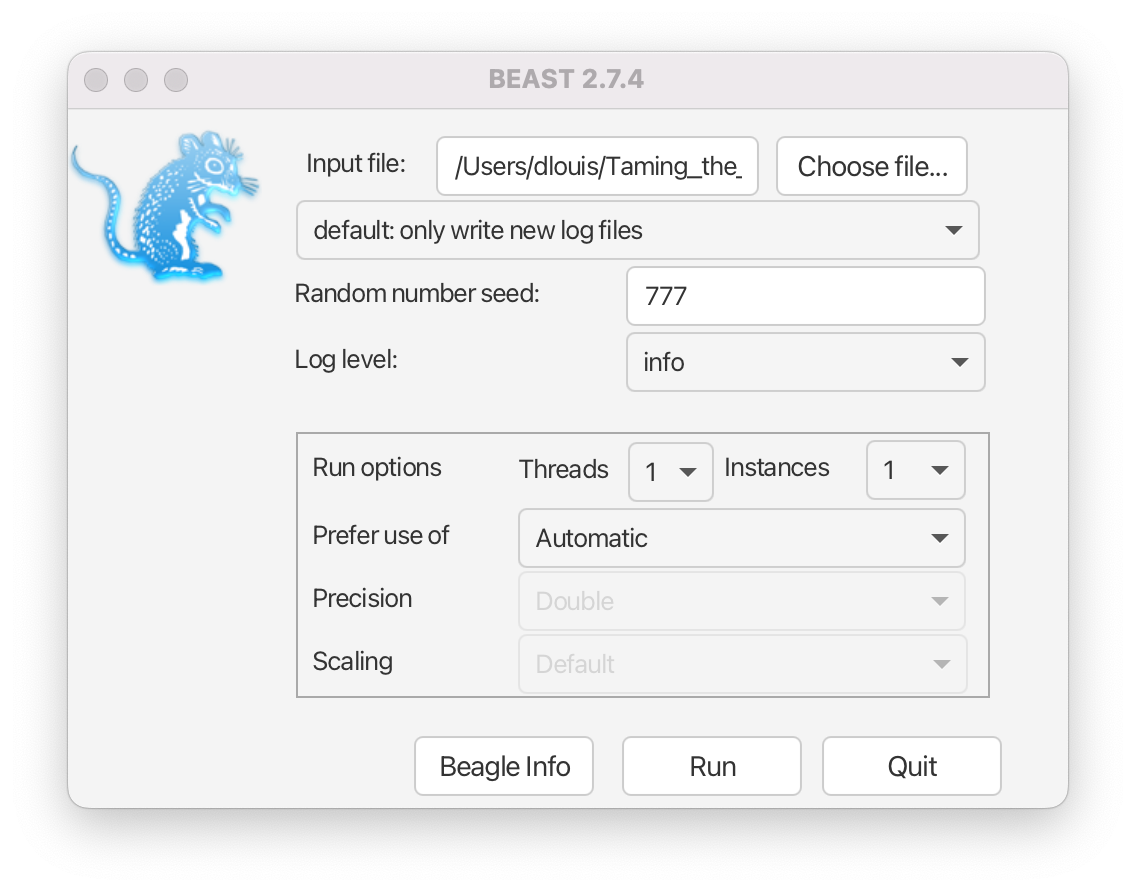
\includegraphics[width=0.800000\textwidth]{figures/beast.png}
    \caption{BEAST2 setup for the analysis.}
    \label{fig:beast}
\end{figure}

The BEAST2 window should look similar to Figure \ref{fig:beast}.

\begin{framed}
Run \textbf{BEAST2} by clicking the \passthrough{\lstinline!Run!}
button.
\end{framed}

BEAST2 will run until the specified number of steps in the chain is
reached. While it is running, it will print the screenlog values to a
console and store the tracelog and tree log values to files located in
the same folder as the configuration XML file. The screen output will
look approximately as shown in Figure \ref{fig:beast_out}.

\begin{figure}
    \centering
    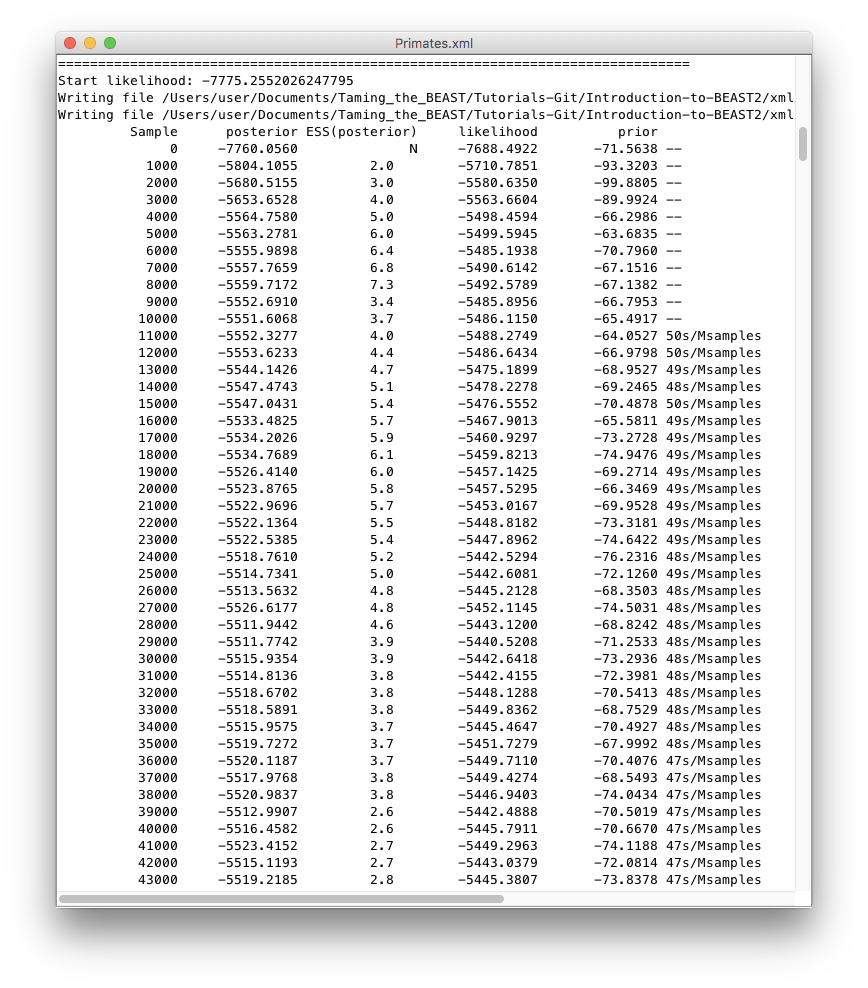
\includegraphics[width=0.800000\textwidth]{figures/beast_out.png}
    \caption{BEAST2 screen output for the analysis.}
    \label{fig:beast_out}
\end{figure}

The window will remain open when BEAST2 finished running the analysis.
When you try to close it, you may see BEAST2 asking the question: ``Do
you wish to save?''. Note that your log and trees files are always
saved, no matter what answer you choose for this question. Thus, the
question is only restricted to saving the BEAST2 screen output (which
contains some information about the hardware configuration, initial
values, operator acceptance rates and running time that are not stored
in the other output files).

\begin{framed}
\textbf{Topic for discussion:} While the analysis is running see if you
can identify which parts of the setup in BEAUti are concerned with the
data, the model and the MCMC algorithm.

Open the XML file in your favourite text editor. Can you recognize any
of the values you set in BEAUti? Can you identify the data, model
specification and MCMC settings in the XML file?

Can you find the likelihood, priors and hyperpriors in the XML file?
\end{framed}

\clearpage

\hypertarget{analysing-the-results}{%
\subsection{Analysing the results}\label{analysing-the-results}}

Once BEAST2 has finished running, open Tracer to get an overview of
BEAST2 output. When the main window has opened, choose
\passthrough{\lstinline!File > Import Trace File...!} and select the
file called \passthrough{\lstinline!primate-mtDNA.log!} that BEAST2 has
created, or simply drag the file from the file manager window into
Tracer.

\begin{framed}
Open \textbf{Tracer}. Drag and drop the
\passthrough{\lstinline!primate-mtDNA.log!} file that BEAST2 created
into the open Tracer window.

Alternatively, use \textbf{File \textgreater{} Import Trace
File\ldots{}} (or press the \textbf{+} button below the \textbf{Trace
Files} panel) then locate and click on
\passthrough{\lstinline!primate-mtDNA.log!}.
\end{framed}

The Tracer window should look as shown in Figure \ref{fig:tracer_bad}.

\begin{figure}
    \centering
    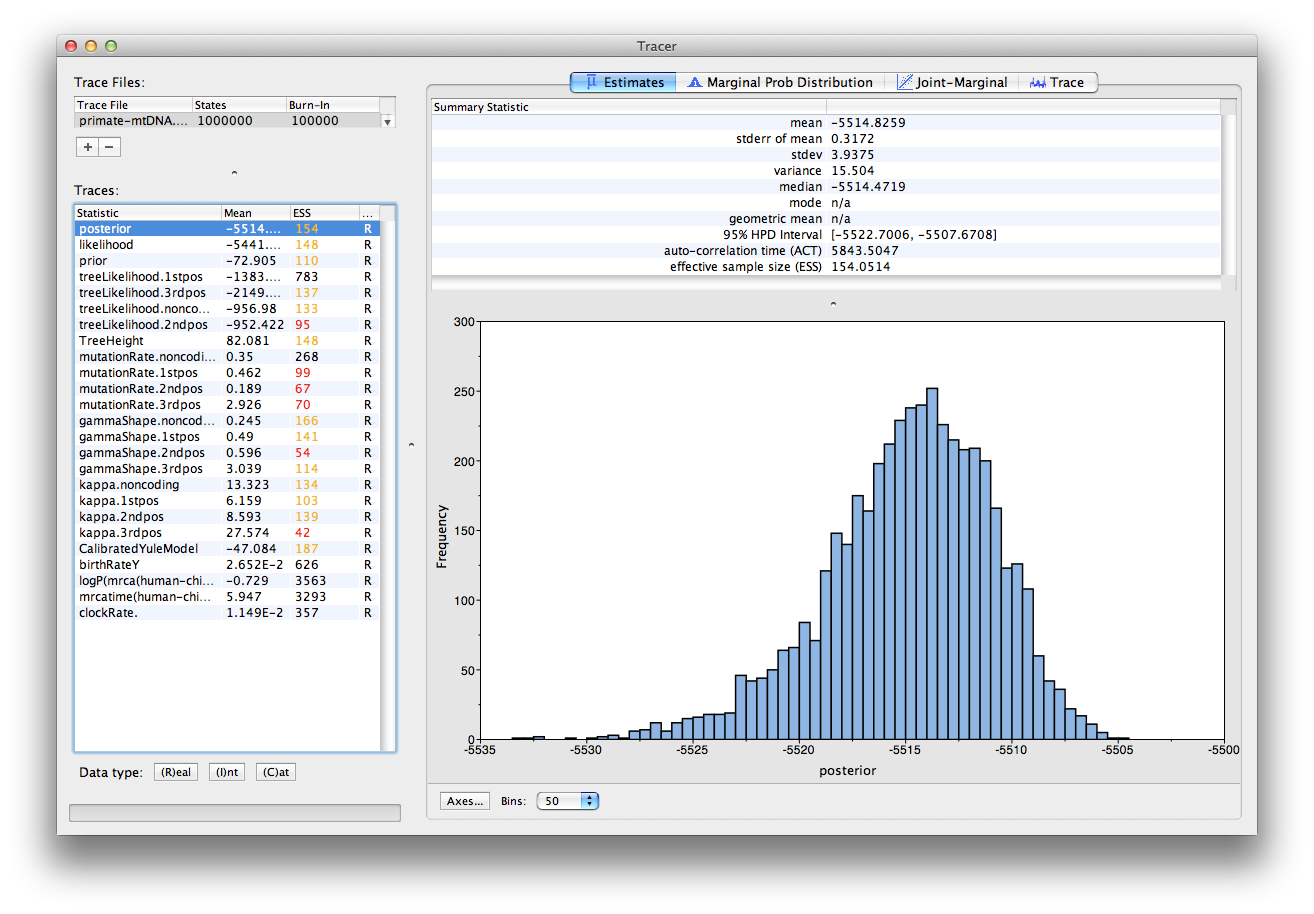
\includegraphics[max width=\textwidth, max height=0.9\textheight]{figures/tracer_bad.png}
    \caption{Tracer showing a summary of the BEAST2 run of primate data with MCMC chain length of 1'000'000.}
    \label{fig:tracer_bad}
\end{figure}

Tracer provides a few useful summary statistics on the results of the
analysis. On the left side in the top window it provides a list of log
files loaded into the program at the moment. The window below shows the
list of statistics logged in each file. For each statistic it gives a
list of summary values such as the mean, standard error, median, and
others it can compute from the data. The summary values are displayed in
the top right window and a histogrom showing the distribution of the
statistic is in the bottom right window.

The log file contains traces for the posterior (this is the natural
logarithm of the product of the tree likelihood and the prior density),
prior, the likelihood, tree likelihoods and other continuous parameters.
Selecting a trace on the left brings up the summary statistics for this
trace on the right hand side. When first opened, the \textbf{posterior}
trace is selected and various statistics of this trace are shown under
the \textbf{Estimates} tab.

For each loaded log file we can specify a \textbf{Burn-In}, which is
shown in the file list table (top left) in Tracer. The burn-in is
intended to give the Markov Chain time to reach its equilibrium
distribution, particularly if it has started from a bad starting point.
A bad starting point may lead to over-sampling regions of the posterior
that actually have very low probability, before the chain settles into
the equilibrium distribution. Burn-in allows us to simply discard the
first \emph{N} samples of a chain and not use them to compute the
summary statistics. Determining the number of samples to discard is not
a trivial problem and depends on the size of the dataset, the complexity
of the model and the length of the chain. A good rule of thumb is to
always throw out at least the first 10\% of the whole chain length as
the burn-in (however, in some cases it may be necessary to discard as
much as 50\% of the MCMC chain).

Select the \textbf{TreeHeight} statistic in the left hand list to look
at the tree height estimated jointly for all partitions in the
alignment. Tracer plots the (marginal posterior) histogram for the
selected statistic and also give you summary statistics such as the mean
and median. The 95\% HPD stands for \emph{highest posterior density
interval} and represents the most compact interval on the selected
statistic that contains 95\% of the posterior density. It can be loosely
thought of as a Bayesian analogue to a confidence interval. The
\textbf{TreeHeight} statistic gives the marginal posterior distribution
of the age of the root of the entire tree (that is, the tMRCA).

\begin{framed}
Select \textbf{TreeHeight} in the bottom left hand list in Tracer and
view the different summary statistics on the right.
\end{framed}

You can also compare estimates of different parameters in Tracer. Once a
trace file is loaded into the program you can, for example, compare
estimates of the different mutation rates corresponding to the different
partitions in the alignment.

\begin{framed}
Select all four mutation rates by clicking the first mutation rate
(\textbf{mutationRate.noncoding}), then holding \textbf{Shift} and
clicking the last mutation rate (\textbf{mutationRate.3rdpos}).

Select the \textbf{Marginal Density} tab on the right to view the four
distributions together.

Select different options in the \textbf{Display} drop-down menu to
display the posterior distributions in different ways.
\end{framed}

You will be able to see all four distributions in one plot, similar to
what is shown in Figure \ref{fig:tracer_comparison}.

\begin{figure}
    \centering
    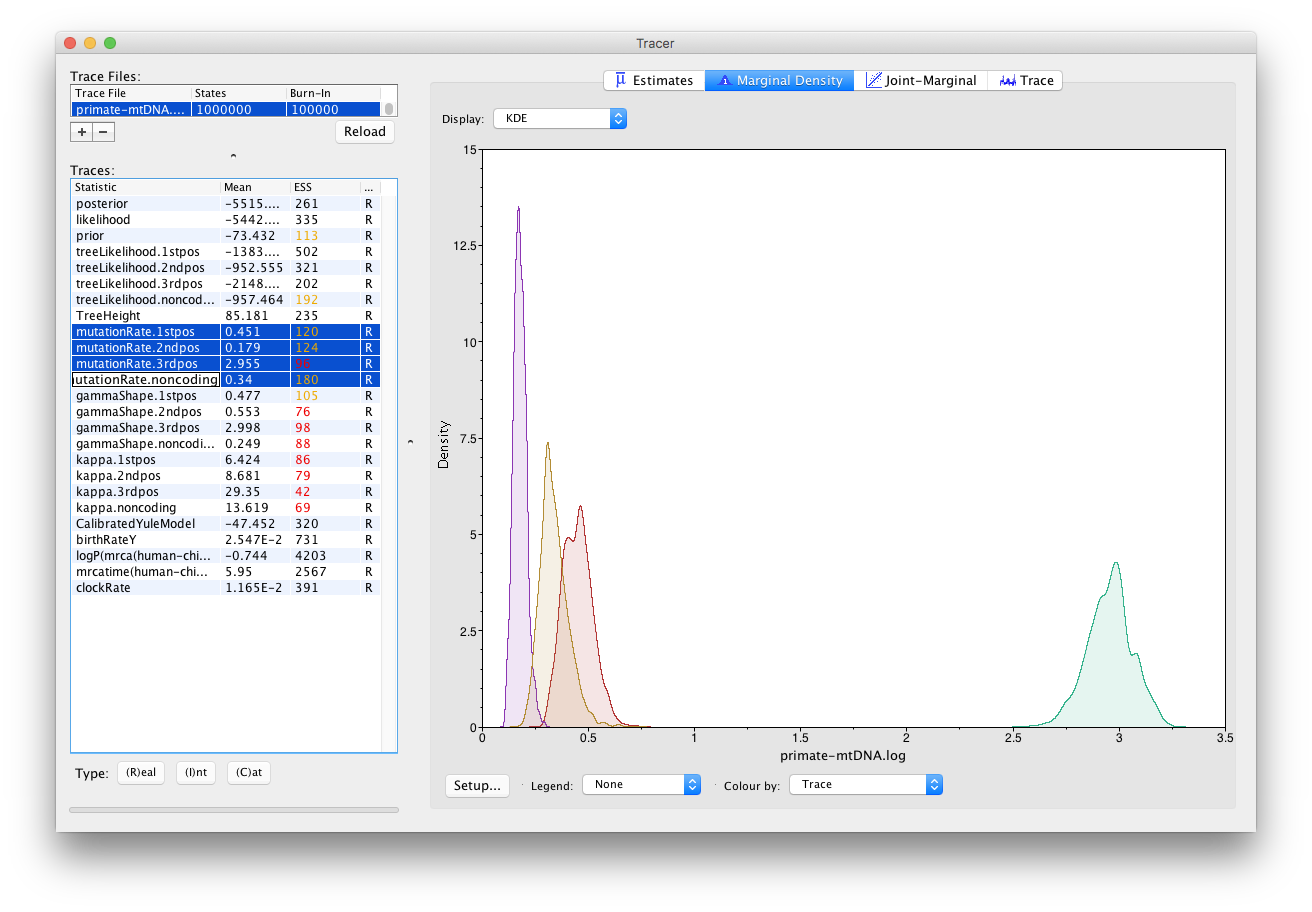
\includegraphics[max width=\textwidth, max height=0.9\textheight]{figures/Tracer_comparison_KDE.png}
    \caption{Tracer showing the four marginal probability distributions of the mutation rates in each partition of the alignment. The figure at the top shows the marginal distributions plotted with a Kernel Density Estimation (KDE) in the middle as violin plots and at the bottom as box and whisker plots.}
    \label{fig:tracer_comparison}
\end{figure}

\begin{framed}
\textbf{Topic for discussion:} What can you deduce from the marginal
densities of the 4 mutation rates? Does this make biological sense?

Why do you think the mutation rate of non-coding DNA is similar to the
rates of 1st and 2nd codon positions? (display the legend on the plot to
help with your analysis).
\end{framed}

\hypertarget{analysing-the-posterior-estimate-quality}{%
\subsubsection{Analysing the posterior estimate
quality}\label{analysing-the-posterior-estimate-quality}}

Two very important summary statistics that we should pay attention to
are the Auto-Correlation Time (ACT) and the Effective Sample Size (ESS).
ACT is the average number of states in the MCMC chain that two samples
have to be separated by for them to be uncorrelated, i.e.~for them to be
independent samples from the posterior. The ACT is estimated from the
samples in the trace (excluding the burn-in). The ESS is the number of
independent samples that the trace is equivalent to. This is calculated
as the chain length (excluding the burn-in) divided by the ACT.

The ESS is in general regarded as a quality-measure of the resulting
sample sequence. It is unclear how to determine exactly how large should
the ESS be for an analysis to be trustworthy. In general, an ESS of 200
is considered high enough to make the analysis useful. However, this is
an arbitrary number and you should always use your own judgment to
decide if the analysis has converged or not. As you can see in Figure
\ref{fig:tracer_bad}, ESS values below 100 are coloured in red, which
means that we should not trust the value of the statistics, and ESS
values between 100 and 200 are coloured in yellow.

If a lot of statistics have red or yellow coloured ESS values, we have
not sufficiently explored the posterior space. This is most likely a
result of the chain not running long enough. Try running the same
analysis as before, but with a longer chain.

\begin{framed}
First load the XML configuration file into BEAUti again by pressing
\textbf{File \textgreater{} Load} and select the
\passthrough{\lstinline!primate-mtDNA.xml!} file. Within BEAUti, change
the MCMC chain length parameter to \textbf{10'000'000} and change the
\textbf{tracelog} frequency to \textbf{1'000}.

Change the trace and tree log file names in order to not overwrite the
results of the previous analysis. You may add something like
\passthrough{\lstinline!\_long!} behind the name of the file, to obtain
\passthrough{\lstinline!primate-mtDNA\_long.log!} for the log file and
\passthrough{\lstinline!primate-mtDNA\_long.trees!} for trees file.

Run BEAST2 again with the updated configuration file and the same seed
of \textbf{777}.
\end{framed}

This will take a bit more time. Figure \ref{fig:tracer_better} shows the
estimates from a longer run. In this case all parameters have ESS values
larger than 200. Remember that MCMC is a stochastic algorithm, so if you
set a different seed the actual numbers will not be exactly the same as
those depicted in the figure.

\begin{figure}
    \centering
    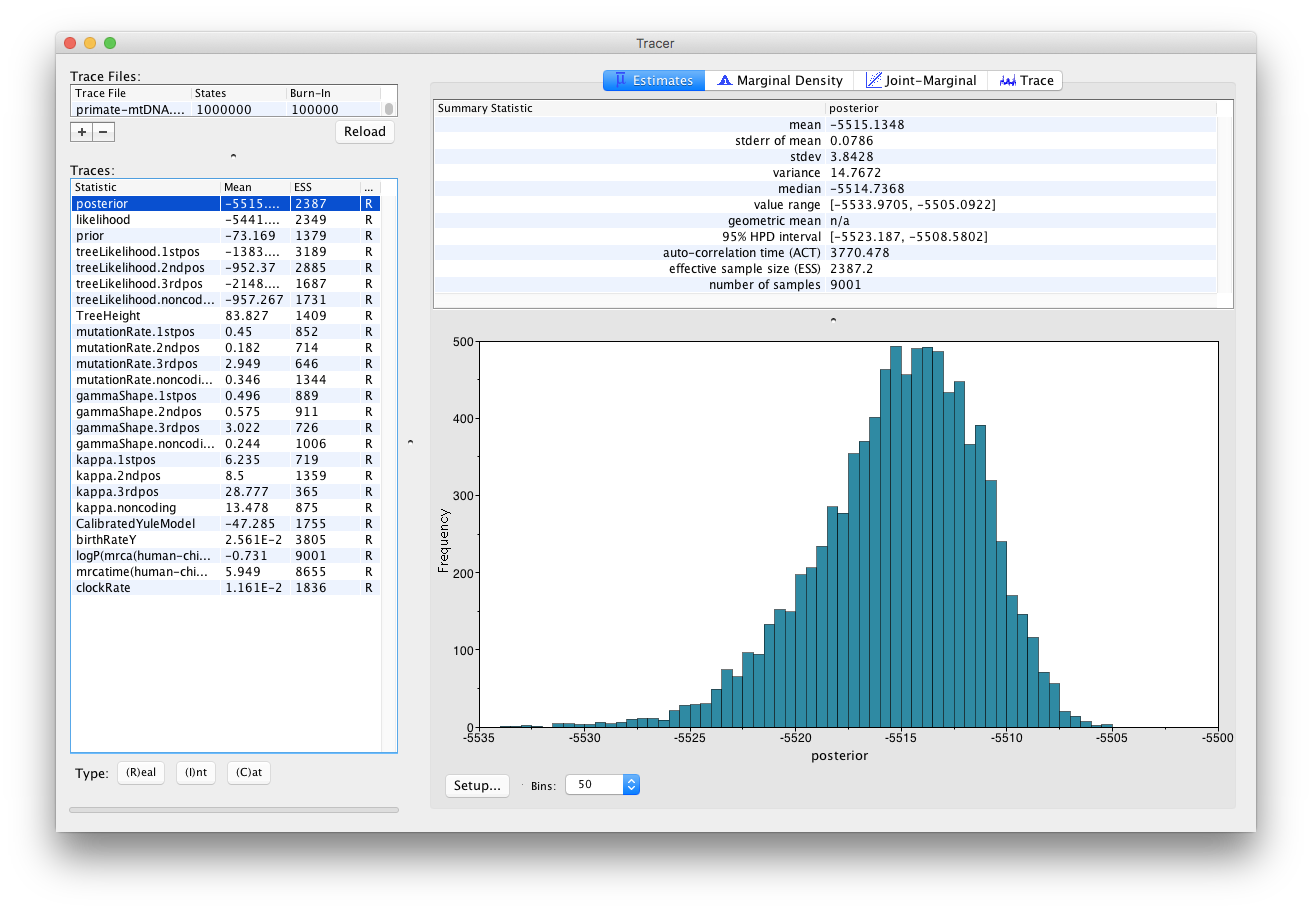
\includegraphics[max width=\textwidth, max height=0.9\textheight]{figures/tracer_good.png}
    \caption{Tracer showing a summary of the BEAST2 run with MCMC chain length of 10'000'000.}
    \label{fig:tracer_better}
\end{figure}

Tracer also allows us to look for correlations between parameters under
the \textbf{Joint Marginal} tab, as shown in Figure
\ref{fig:tracer_joint}. When two parameters are highly correlated this
can lead to poor convergence of the MCMC chain (more on this in later
tutorials).

\begin{figure}
    \centering
    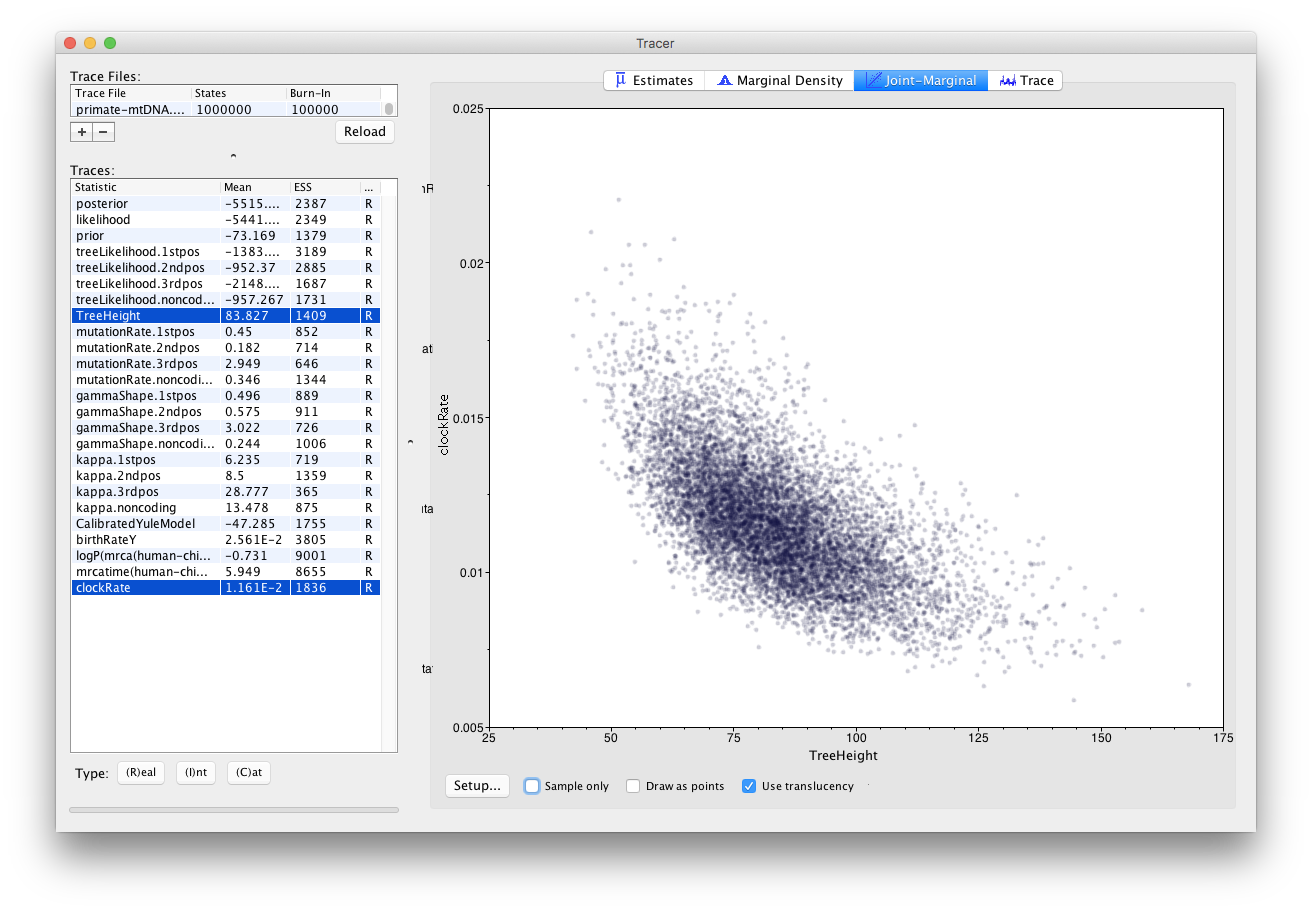
\includegraphics[max width=\textwidth, max height=0.9\textheight]{figures/tracer_joint.png}
    \caption{Correlation between the tree height and clock rate estimates.}
    \label{fig:tracer_joint}
\end{figure}

We can also look at correlations between more than two parameters.

\begin{framed}
Select all 4 mutation rates again

\begin{itemize}

\item
  Navigate to the \textbf{Joint Marginal} tab
\item
  Check \textbf{Show points}
\end{itemize}
\end{framed}

The panel should like Figure \ref{fig:tracer_covariance}. The ellipses
represent the covariance between pairs of parameters and make it easy to
identify which pairs are correlated or anti-correlated. Is there a
strong correlation or anti-correlation between some of our mutation rate
parameters?

\begin{figure}
    \centering
    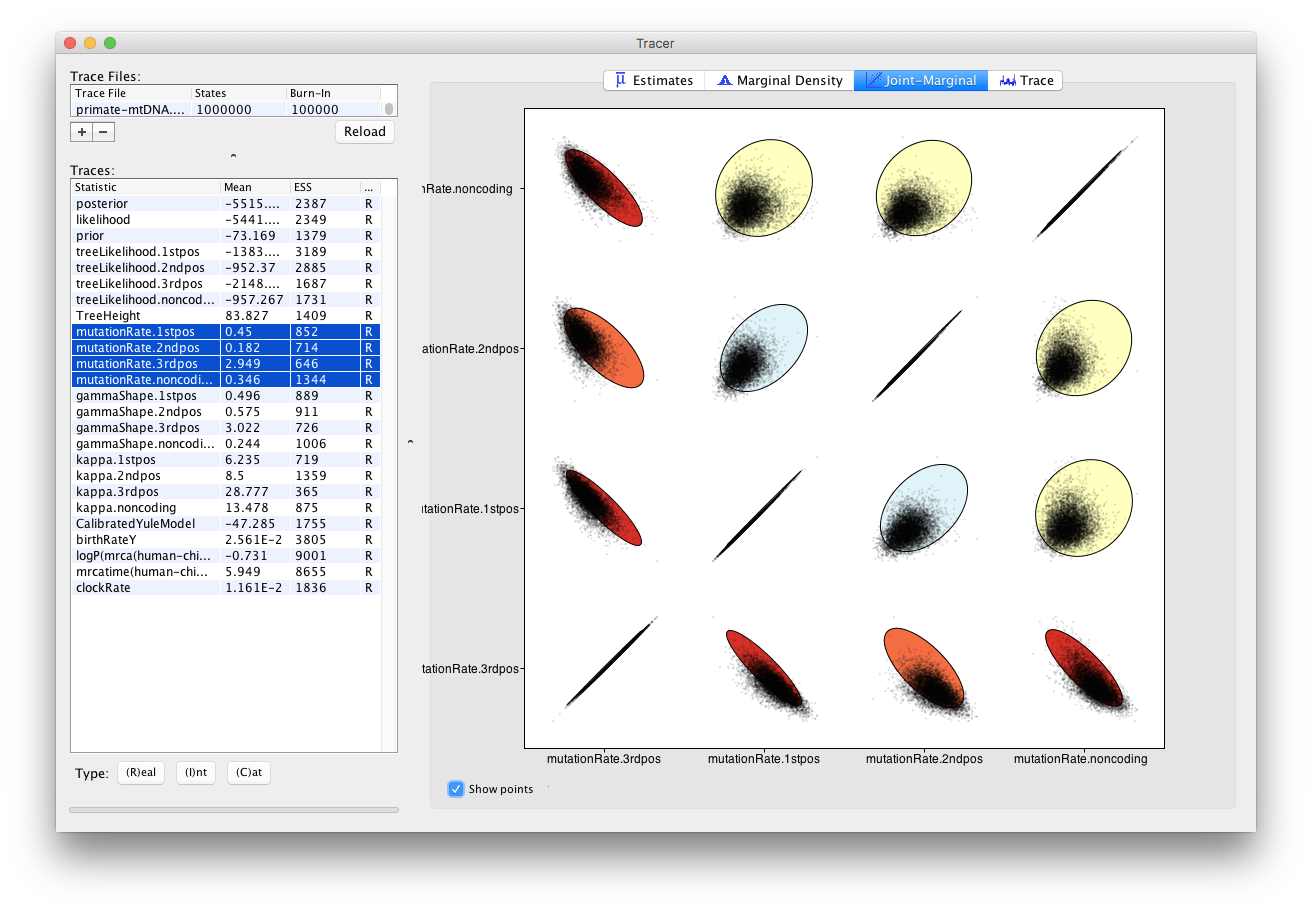
\includegraphics[max width=\textwidth, max height=0.9\textheight]{figures/tracer_covariance.png}
    \caption{Correlations between the mutation rate parameters.}
    \label{fig:tracer_covariance}
\end{figure}

\begin{framed}
\textbf{Topic for discussion:} We have not explored the \textbf{Trace}
tab in Tracer at all!

The \textbf{Trace} tab is primarily a diagnostic tool for checking
convergence to the posterior, assessing the length of the burn-in and
whether or not the chain is mixing well. There is a good argument to be
made for this being the \emph{most important} tab in the Tracer program
and that it is the first tab users should look at.

Have a look at the individual parameter traces in the \textbf{Trace}
tab, in both the short and long log files. Can you figure out why ESS
values for some parameters are higher than others?

Do you think a burn-in of 10\% is sufficient for this analysis?
\end{framed}

\hypertarget{analysing-tree-estimates}{%
\subsubsection{Analysing tree
estimates}\label{analysing-tree-estimates}}

Besides producing a sample of parameter estimates, BEAST2 also produces
a posterior sample of phylogenetic time-trees. These need to be
summarised too before any conclusions about the quality of the posterior
estimate can be made.

One way to summarise the trees is by using the program TreeAnnotator.
This will take the set of trees and find the best supported tree. It
will then annotate this representative summary tree with the mean ages
of all the nodes and the corresponding 95\% HPD ranges. It will also
calculate the posterior clade probability for each node. Such a tree is
called the \emph{maximum clade credibility} tree.

\begin{framed}
Open \textbf{TreeAnnotator}.

Set the \textbf{Burnin percentage} to \textbf{10\%} to discard the first
10\% of trees in the log file.
\end{framed}

The next option, the \textbf{Posterior probability limit}, specifies a
limit such that if a node is found at less than this frequency in the
sample of trees (i.e.~has a posterior probability less than this limit),
it will not be annotated. For example, setting it to 0.5 means that only
nodes seen in the majority (more than 50\%) of trees will be annotated.
The default value is 0, which we will leave as is, and which means that
TreeAnnotator will annotate all nodes.

\begin{framed}
Leave the \textbf{Posterior probability limit} at the default value of
\textbf{0}.
\end{framed}

For the \textbf{Target tree type} option you can either choose a
specific tree from a file or ask TreeAnnotator to find a tree in your
sample. The default option which we will leave, \textbf{Maximum clade
credibility tree}, finds the tree with the highest product of the
posterior probability of all its nodes.

\begin{framed}
Leave the \textbf{Target tree type} at the default value of
\textbf{Maximum clade credibility tree}.
\end{framed}

Next, select \textbf{Mean heights} for the \textbf{Node heights}. This
sets the heights (ages) of each node in the tree to the mean height
across the entire sample of trees for that clade.

\begin{framed}
Select \textbf{Mean heights} in the \textbf{Node heights} drop-down
menu.
\end{framed}

Finally, we have to select the input tree log file and set an output
file.

\begin{framed}
Click \textbf{Choose File} next to \textbf{Input Tree File} and choose
\passthrough{\lstinline!primate-mtDNA.trees!}.

Set the \textbf{Output File} to
\passthrough{\lstinline!Primates.MCC.tree!}.
\end{framed}

The setup should look as shown in Figure \ref{fig:treeannot}. You can
now run the program.

\begin{figure}
    \centering
    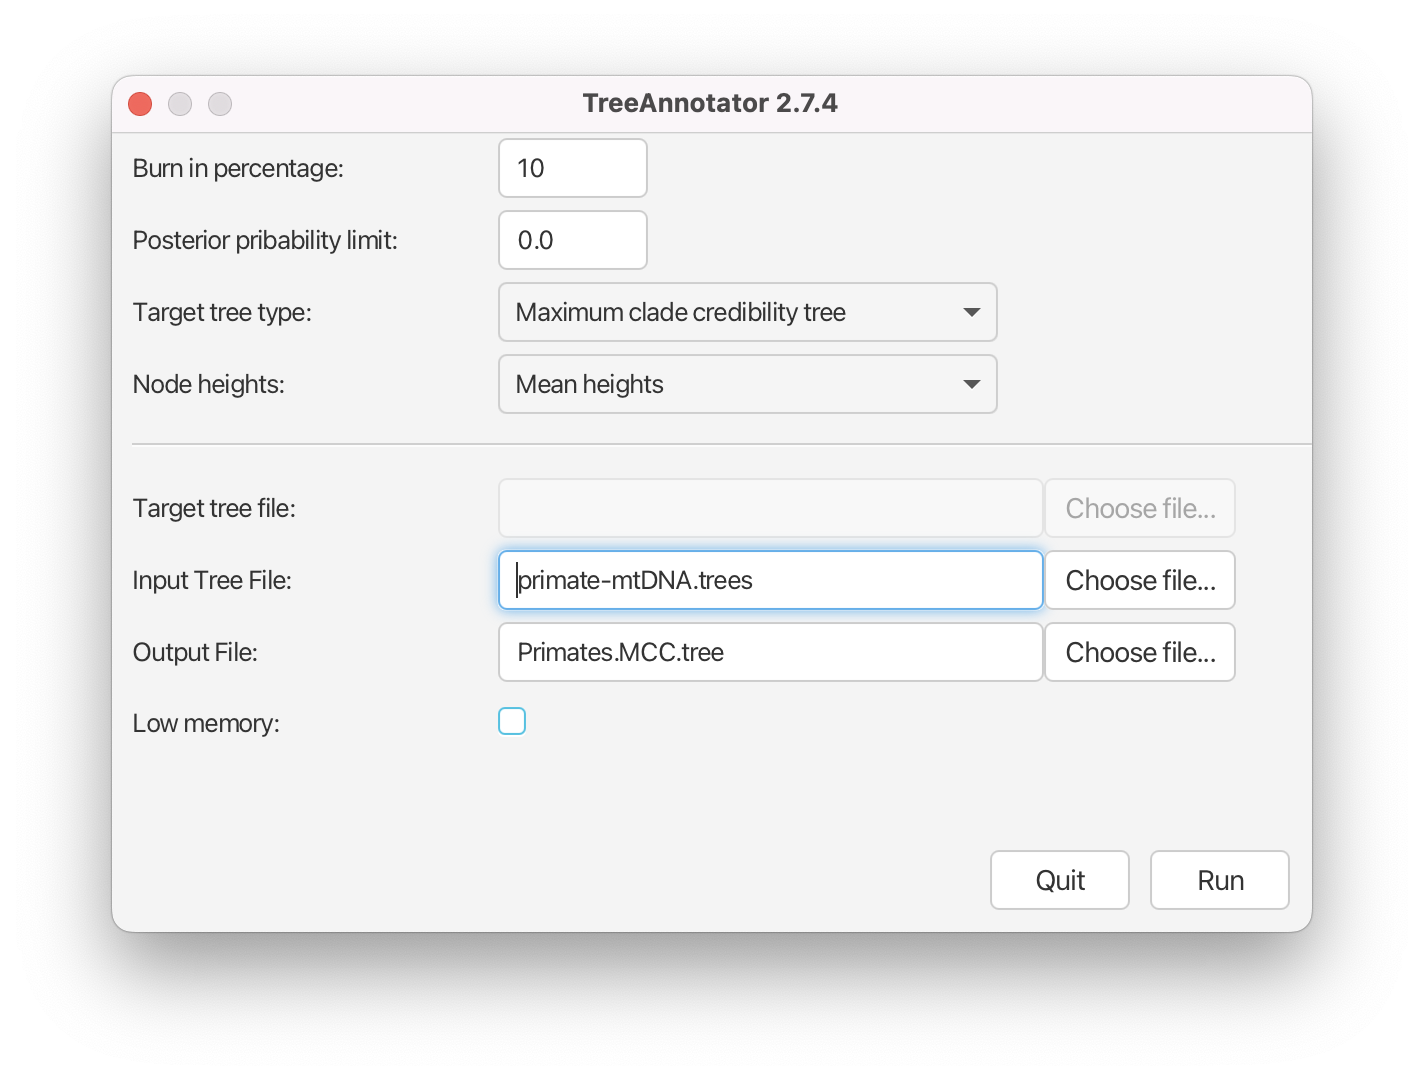
\includegraphics[width=0.800000\textwidth]{figures/treeannot.png}
    \caption{TreeAnnotator setup}
    \label{fig:treeannot}
\end{figure}

\hypertarget{visualising-the-tree-estimate}{%
\subsubsection{Visualising the tree
estimate}\label{visualising-the-tree-estimate}}

Finally, we can visualize the tree with one of the available pieces of
software, such as FigTree.

\begin{framed}
Open \textbf{FigTree}. Use \textbf{File \textgreater{} Open} then locate
and click on \passthrough{\lstinline!Primates.MCC.tree!}.

\begin{itemize}

\item
  Expand \textbf{Trees} options, check \textbf{Order nodes} and select
  \textbf{decreasing} from the drop-down menu.
\item
  Expand the \textbf{Tip Labels} options and increase the \textbf{Font
  Size} until it is readable.
\item
  Check the \textbf{Node Bars} checkbox, expand the options and select
  \passthrough{\lstinline!height\_95\%\_HPD!} from the \textbf{Display}
  drop-down menu.
\item
  Check the \textbf{Node Labels} checkbox, expand the options and select
  \passthrough{\lstinline!posterior!} from the \textbf{Display}
  drop-down menu.
\item
  Increase the \textbf{Font Size} until it is readable.
\item
  Uncheck the \textbf{Scale Bar} checkbox.
\item
  Check the \textbf{Scale Axis} checkbox, expand the options, check
  \textbf{Reverse axis} and increase the \textbf{Font Size}.
\end{itemize}
\end{framed}

\begin{figure}
    \centering
    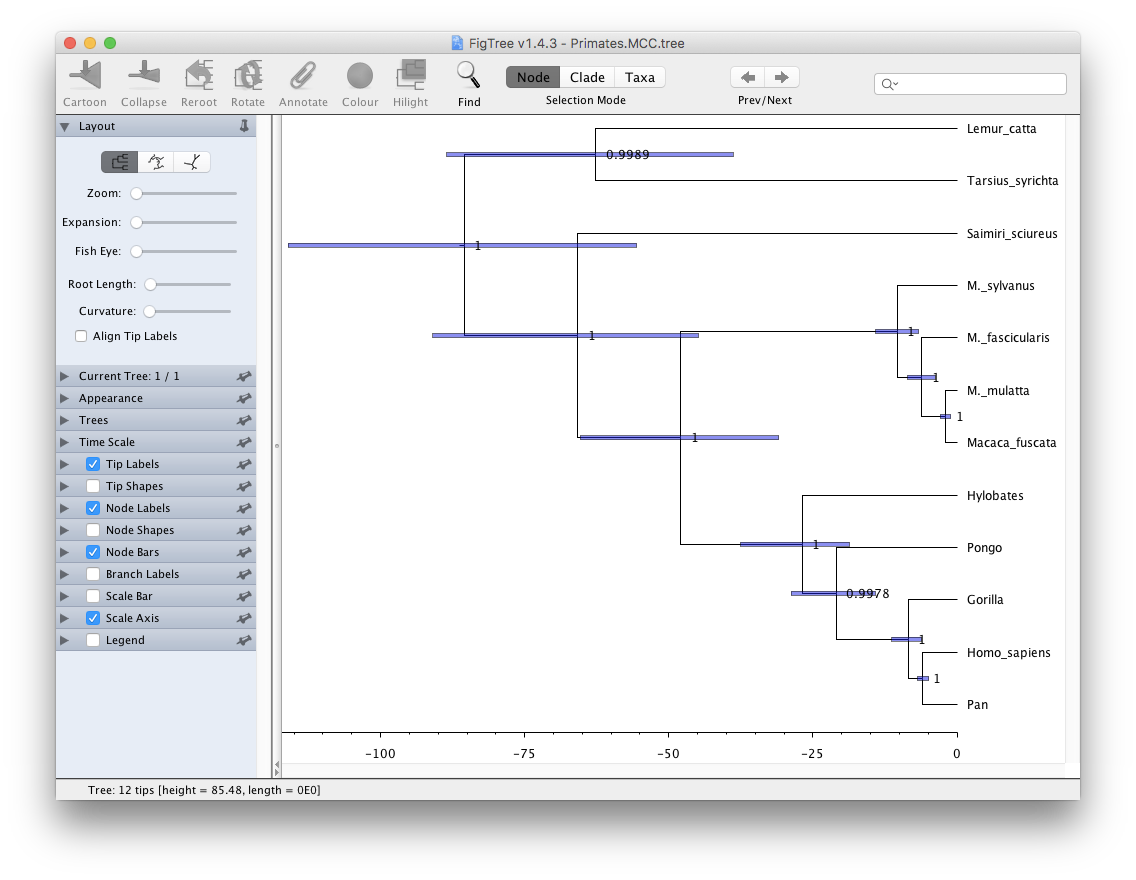
\includegraphics[max width=\textwidth, max height=0.9\textheight]{figures/figtree.png}
    \caption{FigTree visualisation of the estimated tree.}
    \label{fig:figtree}
\end{figure}

Your tree should now look something like Figure \ref{fig:figtree}. We
first ordered the tree nodes. Because there are many ways to draw the
same tree ordering nodes makes it easier for us to compare different
trees to each other. The scale bars we added represent the 95\% HPD
interval for the age of each node in the tree, as estimated by the
BEAST2 analysis. The node labels we added gives the posterior
probability for a node in the posterior set of trees (that is, the trees
logged in the tree log file, after discarding the burn-in). We can also
use FigTree to display other statistics, such as the branch lengths, the
95\% HPD interval of a node etc. The exact statistics available will
depend on the model used.

\begin{framed}
\textbf{Topics for discussion:} The posterior probabilities tell us
which clades are highly supported and the scale bars tell us how
confident we are about their divergence times.

\begin{itemize}

\item
  Are all clades well-supported? How about their ages?
\item
  Look at the 95\% HPD interval for the age of the apes
  (\emph{Hylobates, Pongo, Gorilla, Pan} and \emph{Homo sapiens}). Does
  the estimated age agree with your prior knowledge?
\item
  What about the divergence time between old-world and new-world
  monkeys? (\emph{Saimiri sciureus} is the only new-world monkey in this
  dataset).
\end{itemize}
\end{framed}

\hypertarget{visualising-tree-posteriors-optional}{%
\subsubsection{Visualising tree posteriors
(optional)}\label{visualising-tree-posteriors-optional}}

The MCC tree is one way of summarising the posterior distribution of
trees as a single tree, annotated with extra information on some nodes
to represent the uncertainty in the tree estimates. Just as summarising
the posterior distributions of a continuous parameter as a median and
confidence interval throws away a lot of information (such as the shape
of the distribution) a lot of information is lost when summarising a set
of trees as an MCC tree. However, it is significantly more difficult to
visualise the set of posterior trees.

One possibility is to use the program \textbf{DensiTree}. DensiTree does
not need a summary tree (so we do not need to run TreeAnnotator prior to
using DensiTree) to be able to visualise the estimates.

\begin{framed}
Open \textbf{DensiTree}. Use \textbf{File \textgreater{} Load} then
locate and click on \passthrough{\lstinline!primate-mtDNA.trees!}.

Expand the \textbf{Show} options and check the \textbf{Consensus Trees}
checkbox.
\end{framed}

You should now see many lines corresponding to all the individual trees
samples by your MCMC chain. You can also clearly see a pattern across
all of the posterior trees.

\begin{framed}
In order to see the support for the topology, select the
\textbf{Central} view mode.

Now expand the \textbf{Clades} menu, check the \textbf{Show clades}
checkbox and the \textbf{text} checkbox for the \textbf{Support}.
\end{framed}

The tree should look as shown in Figure \ref{fig:densitree}.

\begin{figure}
    \centering
    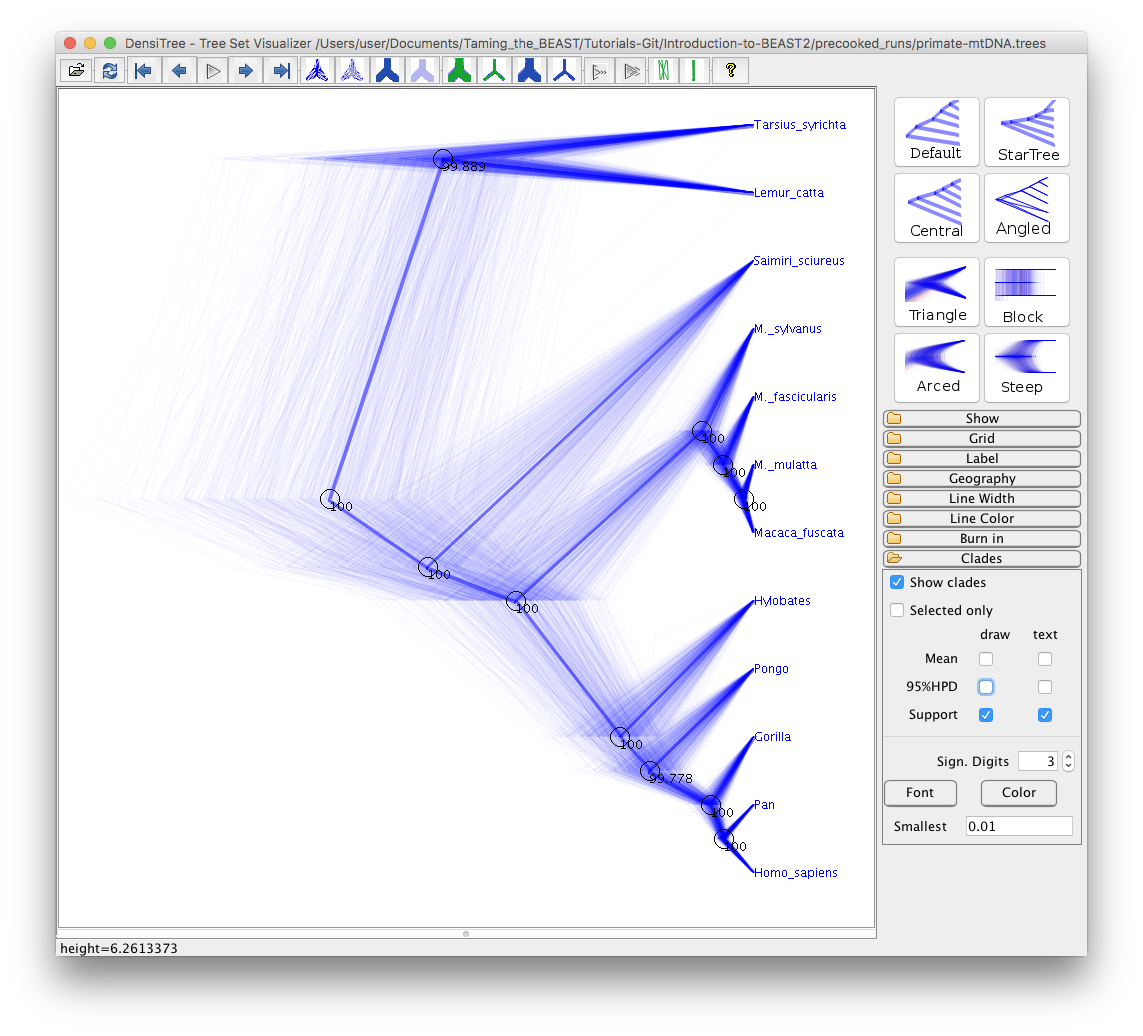
\includegraphics[max width=\textwidth, max height=0.9\textheight]{figures/densitree.png}
    \caption{DensiTree visualisation of the tree sample.}
    \label{fig:densitree}
\end{figure}

You can also view all of the different clades and their posterior
probabilities by selecting \textbf{Help \textgreater{} View clades}. In
this particular run there is little uncertainty in the tree estimate
with respect to clade grouping, as almost every clade has 100\% support.

\begin{framed}
\textbf{Topics for discussion:} The Yule model for speciation has one
parameter (\textbf{birthRateY.t:tree}), representing the speciation
rate. This model assumes that there is no extinction and thus that all
taxa are sampled.

\begin{itemize}

\item
  What are the units for \textbf{birthRateY.t:tree}? From your analysis,
  can you figure out the average time it takes for a speciation event to
  occur? (Have a look at the tracelog).
\item
  Is the Yule model an appropriate model to use here?
\item
  In the dataset there is a much larger sampling proportion for the
  great apes (4/8 extant species) than for lemurs, tarsiers and
  new-world monkeys (one species each). Do you think unequal sampling
  proportions are an issue?
\end{itemize}

\clearpage
\end{framed}

\hypertarget{acknowledgment}{%
\section{Acknowledgment}\label{acknowledgment}}

The content of this tutorial is based on the
\href{https://github.com/CompEvol/beast2/blob/master/doc/tutorials/DivergenceDating/DivergenceDatingTutorialv2.0.3.pdf?raw=true}{Divergence
Dating Tutorial with BEAST 2.0} tutorial by Drummond, Rambaut, and
Bouckaert.

\hypertarget{useful-links}{%
\section{Useful Links}\label{useful-links}}

\begin{itemize}

\item
  \href{http://www.beast2.org/book.html}{Bayesian Evolutionary Analysis
  with BEAST 2} \citep{BEAST2book2014}
\item
  BEAST 2 website and documentation: \url{http://www.beast2.org/}
\item
  BEAST 1 website and documentation:
  \href{http://beast.community}{http://beast.bio.ed.ac.uk}
\item
  Join the BEAST user discussion:
  \url{http://groups.google.com/group/beast-users} \clearpage
\end{itemize}

\hypertarget{relevant-references}{%
}

%%%%%%%%%%%%%%%%%%%%%%%
% Tutorial disclaimer %
%%%%%%%%%%%%%%%%%%%%%%%
% Please do not change the license
% Add the author names and relevant links
% Add any other aknowledgments here
\href{http://creativecommons.org/licenses/by/4.0/}{
\includegraphics[scale=0.8]{figures/ccby.pdf}} This tutorial was written by Jūlija
Pečerska, Veronika Bošková and Louis du
Plessis for \href{https://taming-the-beast.github.io}{Taming the BEAST} and is licensed under a \href{http://creativecommons.org/licenses/by/4.0/}{Creative Commons Attribution 4.0 International License}. 


%%%%%%%%%%%%%%%%%%%%
% Do NOT edit this %
%%%%%%%%%%%%%%%%%%%%
Version dated: \today



\newpage

%%%%%%%%%%%%%%%%
%  REFERENCES  %
%%%%%%%%%%%%%%%%

\printbibliography[heading=relevref]


\end{document}